% !TEX TS-program = XeLaTeX
% all document files must be coded in UTF-8
\documentclass{plateau}

\titlespacing{\section}{0pt}{*1}{*0}
\titlespacing{\subsection}{0pt}{*0}{*0}
\titlespacing{\subsubsection}{0pt}{*0}{*0}

\journalname{PLATEAU}
\thevolume{14}
\thenumber{1}
\theyear{2024}
% DOI

% Cut listings and put github link
% Cut Additional Specifications and put it in github documentation 

\articledoi{10.35699/1983-3652.yyyy.nnnnn}
%\articleid{NNNN} % if the article ID is not the last 5 numbers of its DOI, provide it using \articleid{} commmand
% Abbreviated author list for the running footer
\runningauthor{A. Goyal, A. Potanin and J. Aldrich}
\editorname{Sarah Chasins, Elena Glassman, and Joshua Sunshine}

\title{A Comparative Study of Traditional versus Capability-Based Module
Systems for Modern Programming Languages}
% \othertitle{Subtitle} TODO

% 2 pages - introduction
% 2 pages - background (TODO)
% 1 page - methodology (TODO)
% 3 pages - study designs
% 3 pages - results + conclusion


\author[1]{Abhaas Goyal \orcid{0009-0008-5333-7324}}
\author[2]{Alex Potanin \orcid{0000-0002-4242-2725}}
\author[3]{Jonathan Aldrich \orcid{0000-0003-0631-5591}}

\affil[1, 2]{Australian National University, Australia}
\affil[3]{Carnegie Mellon University, USA}

\addbibresource{refs.bib}

\newcommand{\Eff} {\ensuremath{\mathit{eff}}}  % example command without arguments
\newcommand{\Pre} {\ensuremath{\mathit{pre}}}  % (again)

% Note that you can easily specify arguments:
% \newcommand{\someMacro}[2] {Argument 1: #1, Argument 2: #2} % example command with two arguments
% you use it via \someMacro{Hello}{World!}
\setminted{fontsize=\footnotesize}

% the following commands are being provided by the amsthm package
% the first parameter states the new environmet's name that can be
% used (due to this definition here) and the second the name that
% will appear in the PDF document
\theoremstyle{definition}
\newtheorem{definition}{Definition}   % well, a formal definition!
\theoremstyle{plain}
\newtheorem{prop}{Proposition} % like a theorem, but less important or evolved
\newtheorem{lem}{Lemma}        % used within a proof of a theorem
\newtheorem{thm}{Theorem}      % well, a theorem! :) important and evolved
\newtheorem{cor}{Corollary}    % basically either a proposition or theorem,
                               %  but one that follows from another theorem.
% There's a lot you can configure about the appearance. If interested,
% open the manual of amsthm or google for tutorials etc. on that package

\newmdtheoremenv{hyp}{Hypothesis}

% the following add a symbol to the definition environment to make it more
% clear when a definition ends (as there is no difference in fonts!). From:
% https://tex.stackexchange.com/questions/226334/change-a-amsthm-theorem-ending
\newcommand{\xqed}[1]{%
    \leavevmode\unskip\penalty9999 \hbox{}\nobreak\hfill
    \quad\hbox{\ensuremath{#1}}}
\newcommand{\Endofdef}{\xqed{\blacksquare}}
\newenvironment{defn}[1]{%
    \begin{definition}#1}{%
    \Endofdef\end{definition}%
}

\begin{document}
\maketitle

\begin{abstract}
The principle of least privilege serves as an essential guideline in designing secure computing systems. However, implementing this in real-world systems through various programming languages has proved to be difficult and has allowed for many vulnerabilities in privilege escalation. One proposed solution is to have capability-based security primitives in programming languages for modules and objects. A capability is a unique token that provides the authority to perform a specific set of actions on a selected resource. However, its effectiveness as a language design choice for real-world applications remains to be seen.

To answer this question, we designed a comparative study to compare programmer productivity, security of the designs, and extensibility of packages in capability-based module systems vs.\ others. Our main goal was to determine whether module systems/packages having capabilities from the ground up provide usability and security advantages compared to their absence. The study used two programming languages - one with object capabilities (Wyvern) and the other with support for capabilities via external libraries (Rust).

Preliminary findings show that programs designed in Wyvern provided higher security guarantees in some cases, and users found using object capabilities an easy-to-use secure abstraction layer for managing critical resources. However, a lack of tooling for showing appropriate errors or code completion introduced challenges in writing code. Hence, future work requires a more in-depth study to define and validate current user-centric methods of designing capability-based languages. Further work also involves classifying security vulnerabilities solved by capabilities and building the necessary tools in Wyvern to make capabilities more viable as a design choice in programming languages.

% TODO
\keywords{Object Capabilities \sep Language-based Security \sep Module Systems \sep Rust \sep Wyvern}
\end{abstract}




\section{Introduction}\label{sec-intro}
\noindent
A rise of sophistication in cyber-security attacks has led to increased research in language-based security \cite{10.1007/11555827_12}, which attempts to provide computer security for applications at an architectural level. One of the core principles to follow in their designs is the principle of least privilege - which states that every user and process should be provided with minimal authority over the underlying system resources. 

Initial attempts to achieve authority control in systems centered around two symmetric approaches. \cite{millerKeynote} The first was the identity-centric model, which was implemented using access-controlled lists. The other one was the authority-centric model known as capabilities, which kept designation and authority together. The former became the industry standard for various historical reasons leading to myths around using capabilities in production systems \cite{markCapsMyth}. 

The Open Worldwide Application Security Project (OWASP) provides a regularly updated list of the top 10 list of "most critical security risks faced by organizations in web applications" \cite{owaspTop10}. Within the list, \textbf{Broken Access Control} has been put at the number one spot \cite{owaspBrokenAccess}. Several subsets of vulnerabilities exist within this category- such as \textit{Execute Code}, \textit{Directory Traversal}, and \textit{Gaining Privilege}. Recently, research into capabilities has been re-assessed as a potential solution by the research community. Capabilities have been implemented in a wide variety of contexts, such as standard library packages in various programming languages (\cite{rustCap}, \cite{scalaCaps}, \cite{goCap}), Operating Systems such as sel4 \cite{sel4}, and even in hardware architectures \cite{watson2018capability}. 

In addition to building capability-based systems based on libraries, we can design programming languages that use capabilities from the ground up to design secure programs. In the past, this has been attempted both in older languages such as E \cite{eProgLang} and Newspeak \cite{newspeakProgLang}, as well as modern languages such as Pony \cite{steed2016principled} and Wyvern \cite{DBLP:wyvern}.

% \begin{figure}[htbp]
% \centering
% 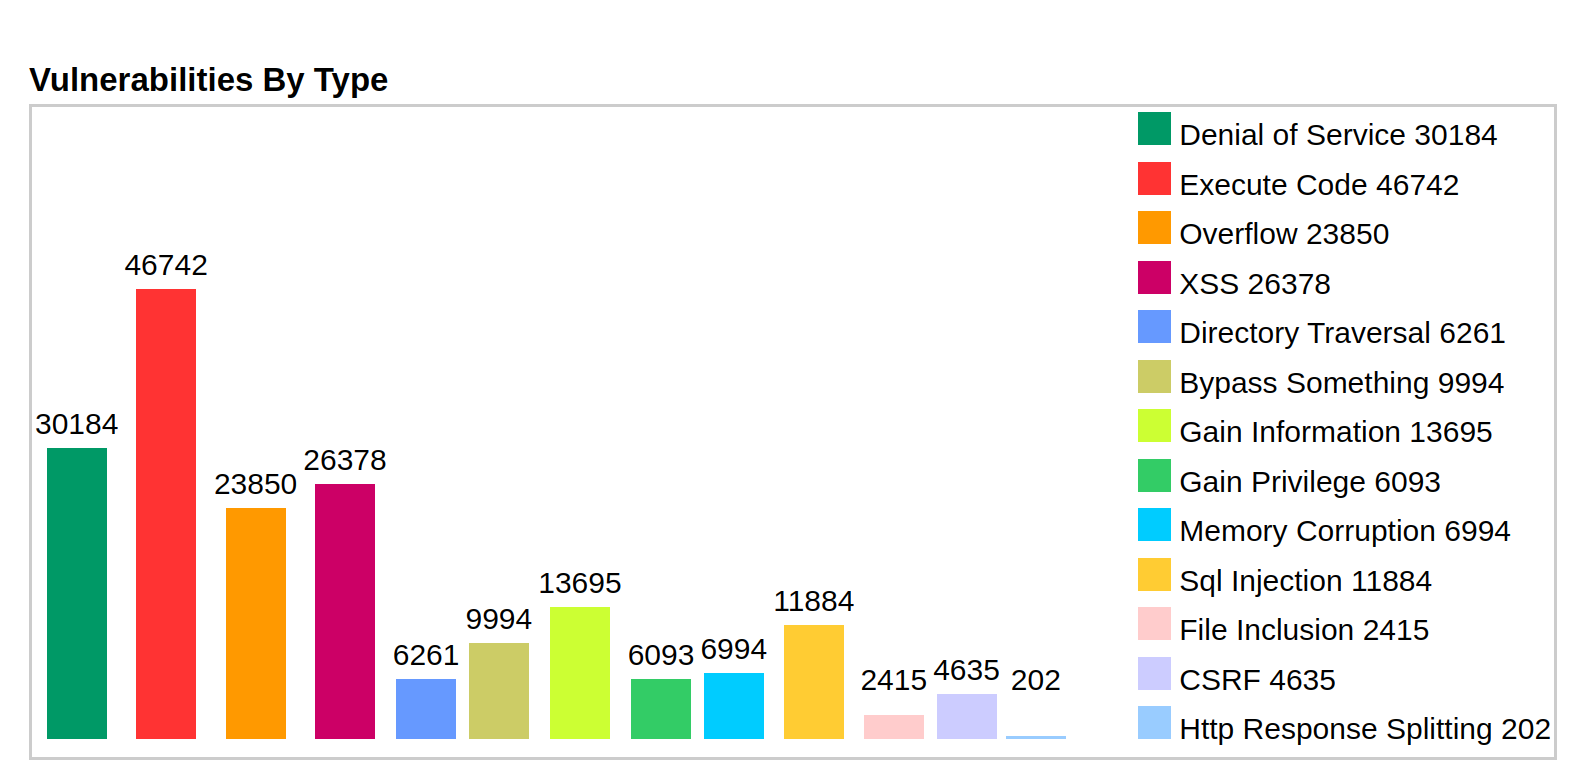
\includegraphics[width=7cm]{./figures/mitre.png}
% \caption{Vulnerabilities by type, classified by MITRE \cite{mitre} }
% \end{figure}

However, it remains to be seen whether regular software developers can use capability-based languages in teams to design applications and the effect of doing so on introduced security vulnerabilities, compared with a library-based approach. To answer this question, we frame the following research questions for the project:

\begin{enumerate}
    \item \textbf{RQ1}: How usable are capability-based languages when designing an architecture?
    \item \textbf{RQ2}: What security vulnerabilities do programmers expose when designing resource-critical objects?  
\end{enumerate}

To answer these questions, we set up a comparative study between two languages - one with object capabilities (Wyvern) and the other with support for capabilities via external libraries (Rust). The two languages were chosen based on the following parameters:

\noindent
\textbf{Reasons to choose Wyvern}
\begin{enumerate}
    \item Provides a capability-based module-system with formalized authority-control \cite{DBLP:journals/darts/MelicherSPA17}. Here, system resources are represented as object capabilities and must explicitly be passed as arguments, limiting access to certain system resources. This feature will help us to design a multi-tiered architecture while controlling security in each layer.
    \item Domain-specific syntax support within the language provides good support for embedding other languages (such as in the case of web development HTML/SQL), so users can have an easier time designing architecture with high safety/security properties.
    \item A potential future scope of the Wyvern project lies in studying the usability and security of Effect Systems in conjunction with capabilities. A comparable language is Koka \cite{leijen2014koka}, but it does not have effects primarily for security reasons since they do not support user-defined, object-based effects.
\end{enumerate}


\noindent
\textbf{Reasons to choose Rust}
\begin{enumerate}
    \item In terms of choosing a capability library among modern languages, the Rust library was found to be the most stable. (Object-Capabilities in Scala \cite{scalaCaps} was another candidate but the library is currently in beta).
    \item Considered as the most loved language on Stack Overflow \cite{rustLove}, so a strong case for increasing future user adoption rates.
    \item Supports multiple paradigms of programming, such as imperative and functional programming, which increases suitability for getting more users for the study.
    \item Systems language with a strong type system, known to be secure due to ownership, so it would be interesting to see security vulnerabilities arising from using this language.
\end{enumerate}

Our findings are in their preliminary stages. They show that programs designed in Wyvern provided higher security guarantees, and users found that object capabilities provided an easy-to-use yet a secure abstraction layer for critical resource management. However, a lack of tooling for showing appropriate errors or code completion introduced ease of use challenges when writing programs. Informed by these findings, future work is required primarily in designing a more in-depth study to understand the user-centric methods needed to design capability-based languages. Further work also involves classifying security vulnerabilities solved by capabilities and building the necessary static analysis tools/debugging aids in Wyvern to make capabilities more viable as a design choice in programming languages.
\section{Background and Related Work}\label{sec-background}


\begin{figure}[htbp]
\begin{minipage}[t]{0.35\textwidth}
\centering
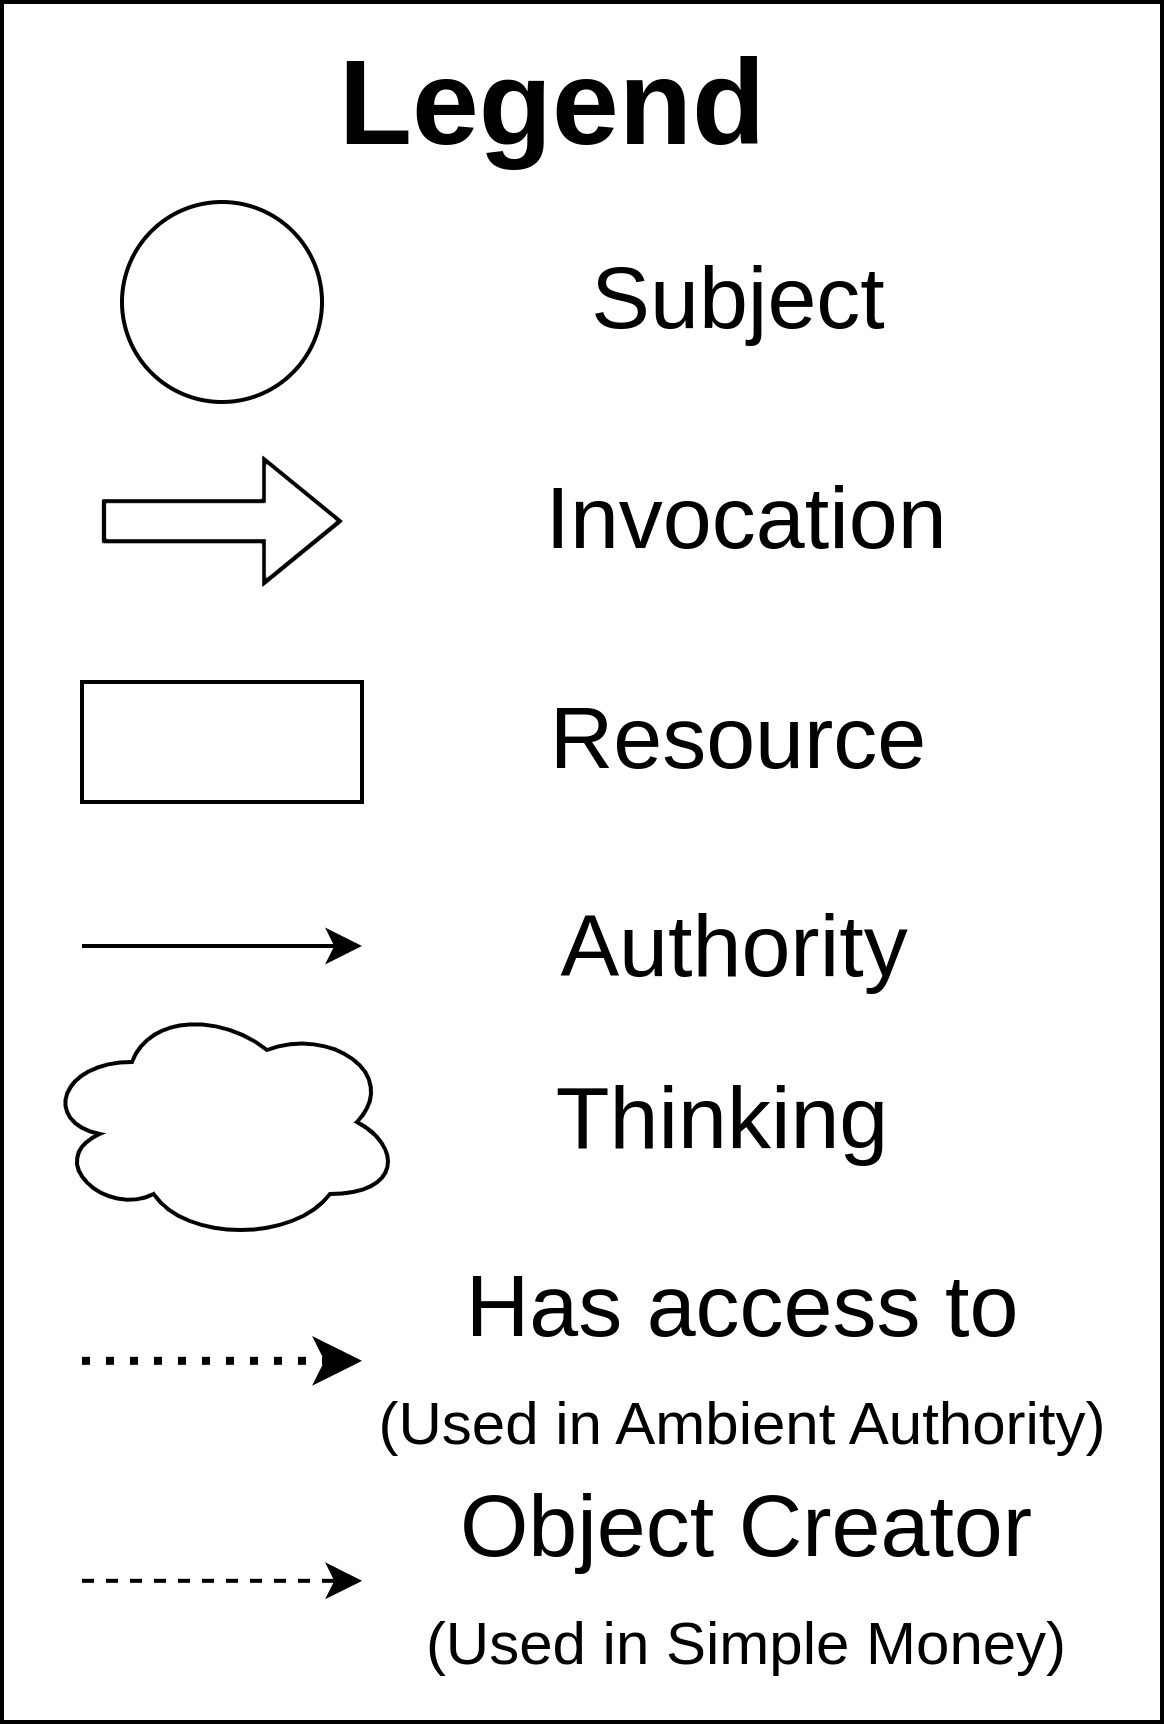
\includegraphics[width=1.4in]{figures/Legend.jpg}
\caption{Legend for various entities in object-capability diagrams}
\end{minipage}
\hspace{\fill}
\begin{minipage}[t]{0.55\textwidth}
\centering
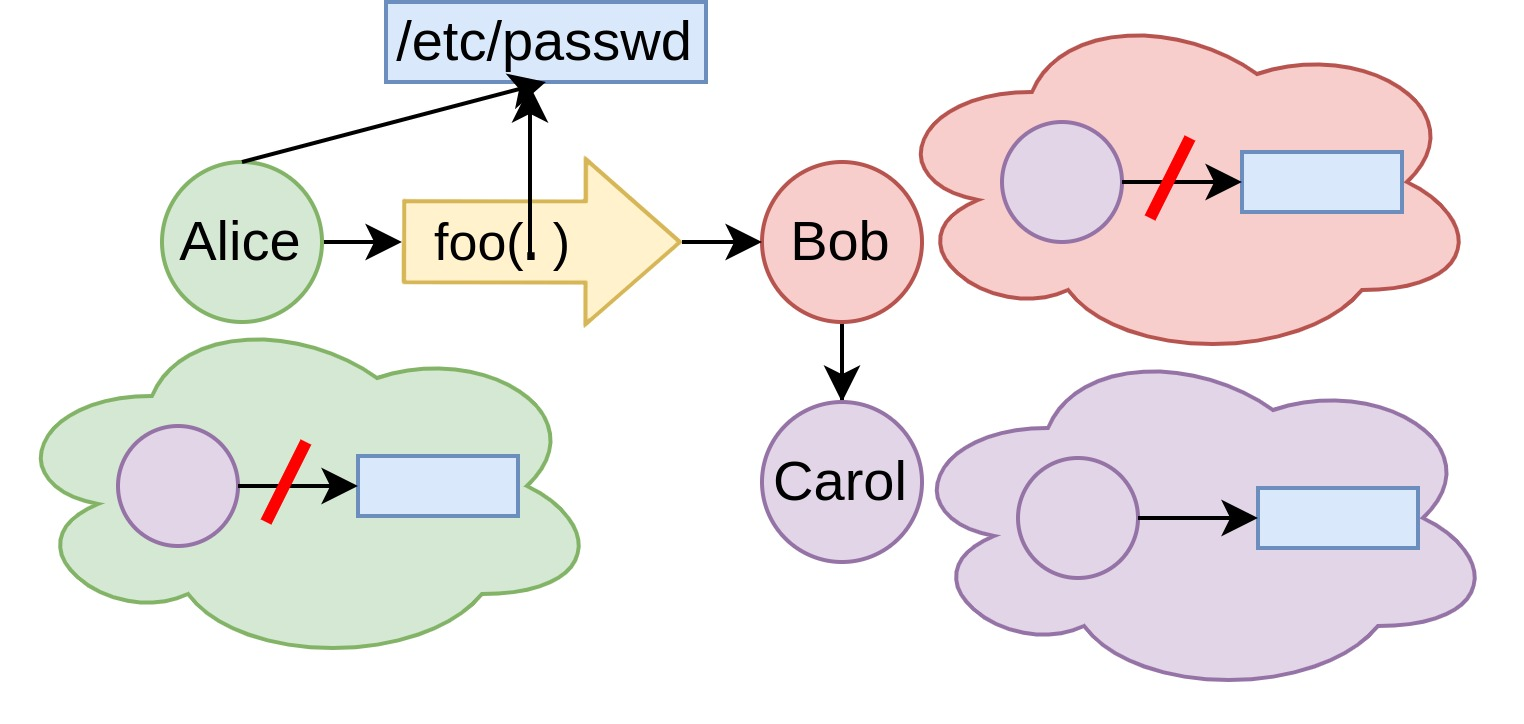
\includegraphics[width=2.8in]{figures/confused_deputy.jpg}
\caption{The Confused Deputy Problem represented as a Granovetter Diagram \cite{millerCapRights}}
\label{cdp}
\end{minipage}
\end{figure}
\noindent
We provide a background on the motivation for using capability-based design and a sample capability pattern used in one of the study designs. 

\subsection{Capabilities: Motivation}
% http://www.cap-lore.com/CapTheory/ConfusedDeputyM.html

\noindent
To start with why we need capabilities, we first need to look at the Confused deputy problem~\cite{millerCapRights}. In Figure \ref{cdp}, Bob acts as the deputy and is deemed trustworthy by every other entity (hence the term ``deputy''). He is communicating with Alice and Carol. Alice then provides Bob with a sensitive resource (in this case \texttt{/etc/passwd} with specific permissions) and trusts Bob enough not to pass the sensitive resource to Carol. The question then arises whether Carol can "trick" Bob into access to the underlying resource, thus leading to broken access control. Currently, many real-world vulnerabilities are present in this class (due to ambient authority) with common examples being Cross-Site Request Forgery (CSRF) \cite{blatz2007csrf} and VSCode extensions (\cite{vscodevuln}).

However, Rust provides module systems that don't have ambient authority, for which one could argue that these bugs would not happen in the future (i.e., we consider Bob won't be pinned as a reason for broken access control). This further propagates the question of whether capabilities as a language design choice by itself provide additional advantages.

\cite{millerCapRights} further discusses object-capabilities security as one of the methods to avoid the confused deputy problem. Capabilities can be viewed as one of the interpretations of the Granovotter diagram. It is defined as the following:

If Bob does not have access to Carol (which is a critical resource), he can only gather access to it from someone else. Let us assume it's Alice; she can only give the resource to Bob only if:
\begin{itemize}
    \item Alice already has the authority to Carol object (via a reference)
    \item Alice has a reference to Bob
    \item (Key part) Alice decides to voluntarily share the reference to Carol with Bob
\end{itemize}

% A brief overview of capabilities is given in the next section.
% Let us use this analogy in implementing the Linux operating system, where access to files is stored in an Access Control List (ACL). If (a) the running process is Bob, (b) Alice has already provided Bob with the necessary permissions to read/write the resource, and (c) Carol has already invoked Bob and is asking for the underlying resource, the underlying OS will only look at the process id of the caller, i.e., Bob, see that it has the necessary permissions, and ultimately return the result to Carol. Here, there exists ambient authority on the \texttt{/etc/passwd}, since one only needs to name the resource and the necessary operation to the right person. 


% https://wiki.c2.com/?ConfusedDeputyProblem
% One could pin the underlying reason onto Bob, saying that its methods called from Carol did not check for the authority itself and thus invoked a security hole. Even though this is true on a high level, considering that the amount of software being written is large, which would lead to more unforced errors, we need to "find a more fundamental cause." Here, the reason is that there is a separation of (a) the underlying reason for Bob's permission and (b) What Bob is actually doing.


% \begin{figure}[htbp]
% \centering
% 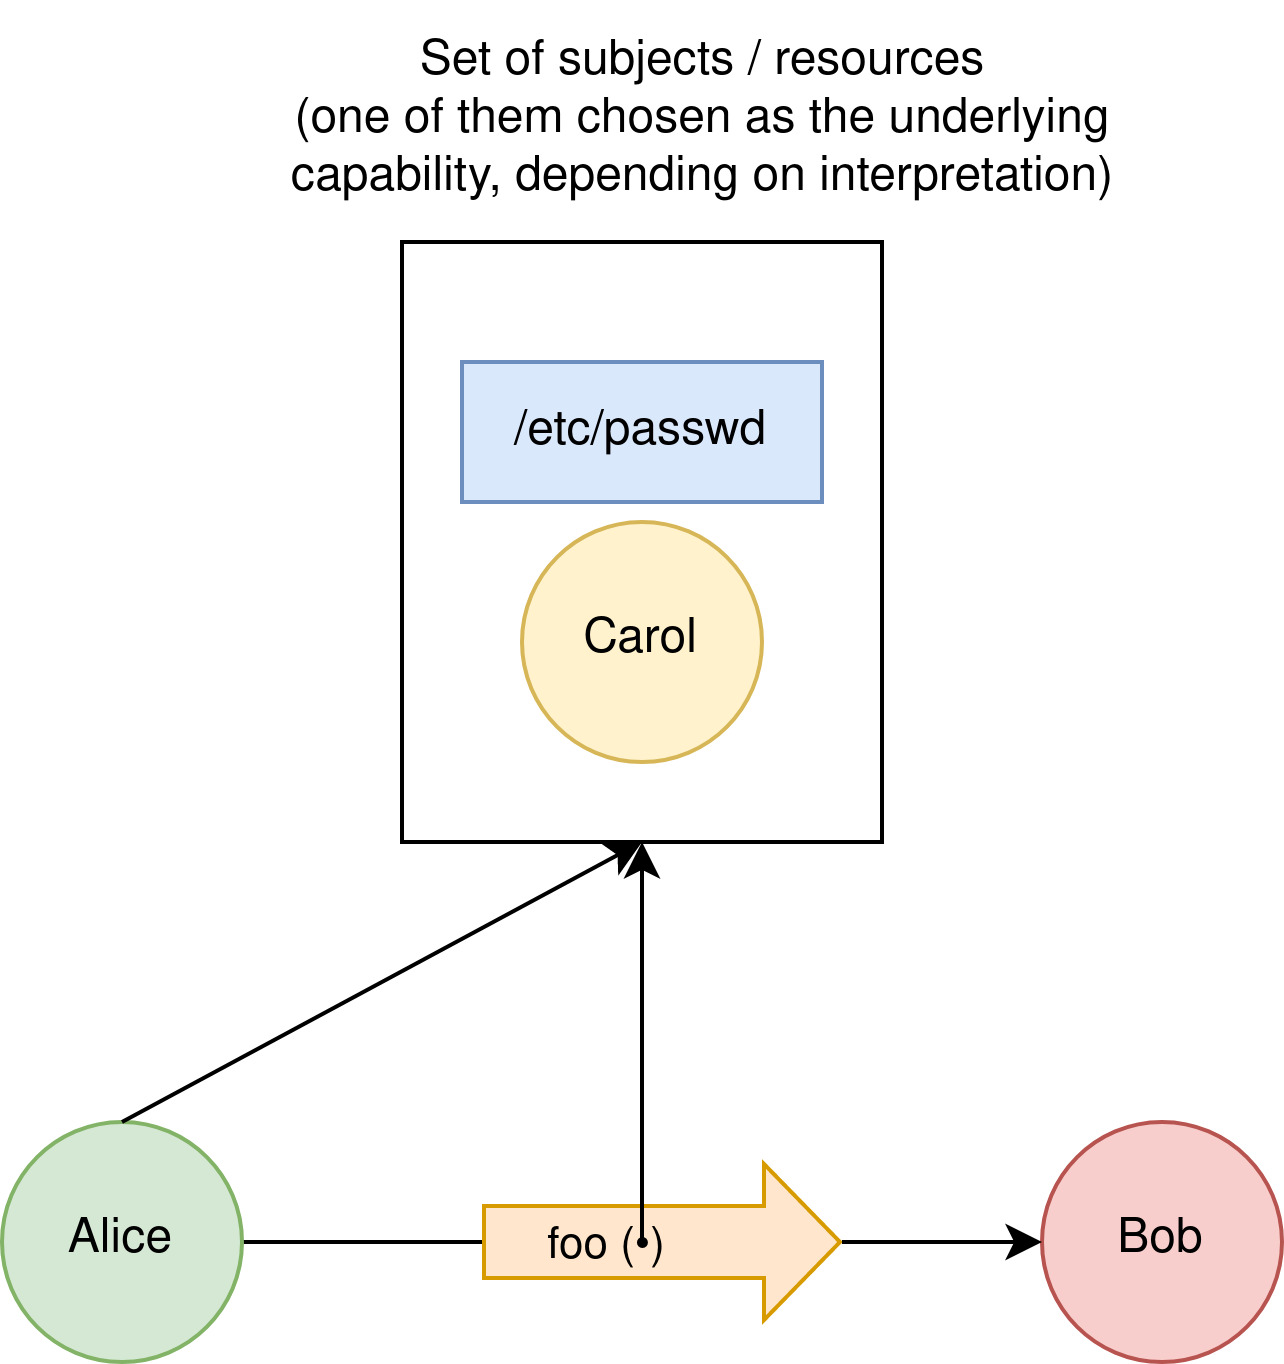
\includegraphics[width=2.5in]{figures/cap.jpg}
% \caption{The Granovetter Diagram viewed as a capability object}
% \end{figure}
% http://erights.org/elib/capability/ode/overview.html

% http://habitatchronicles.com/2017/05/what-are-capabilities/
Capabilities can be summarised as - "Don't separate authority from designation." \cite{markCapsMyth}. The design choice in creating programs with capabilities is for a main trusted program to provide the correct amount of capability (which is implemented as non-forgeable references) to each specific object.  

% Figure \ref{cap_acl} provides a shift in perspective from ACLs to capabilities.

% \begin{figure}[htbp]
% \centering
% 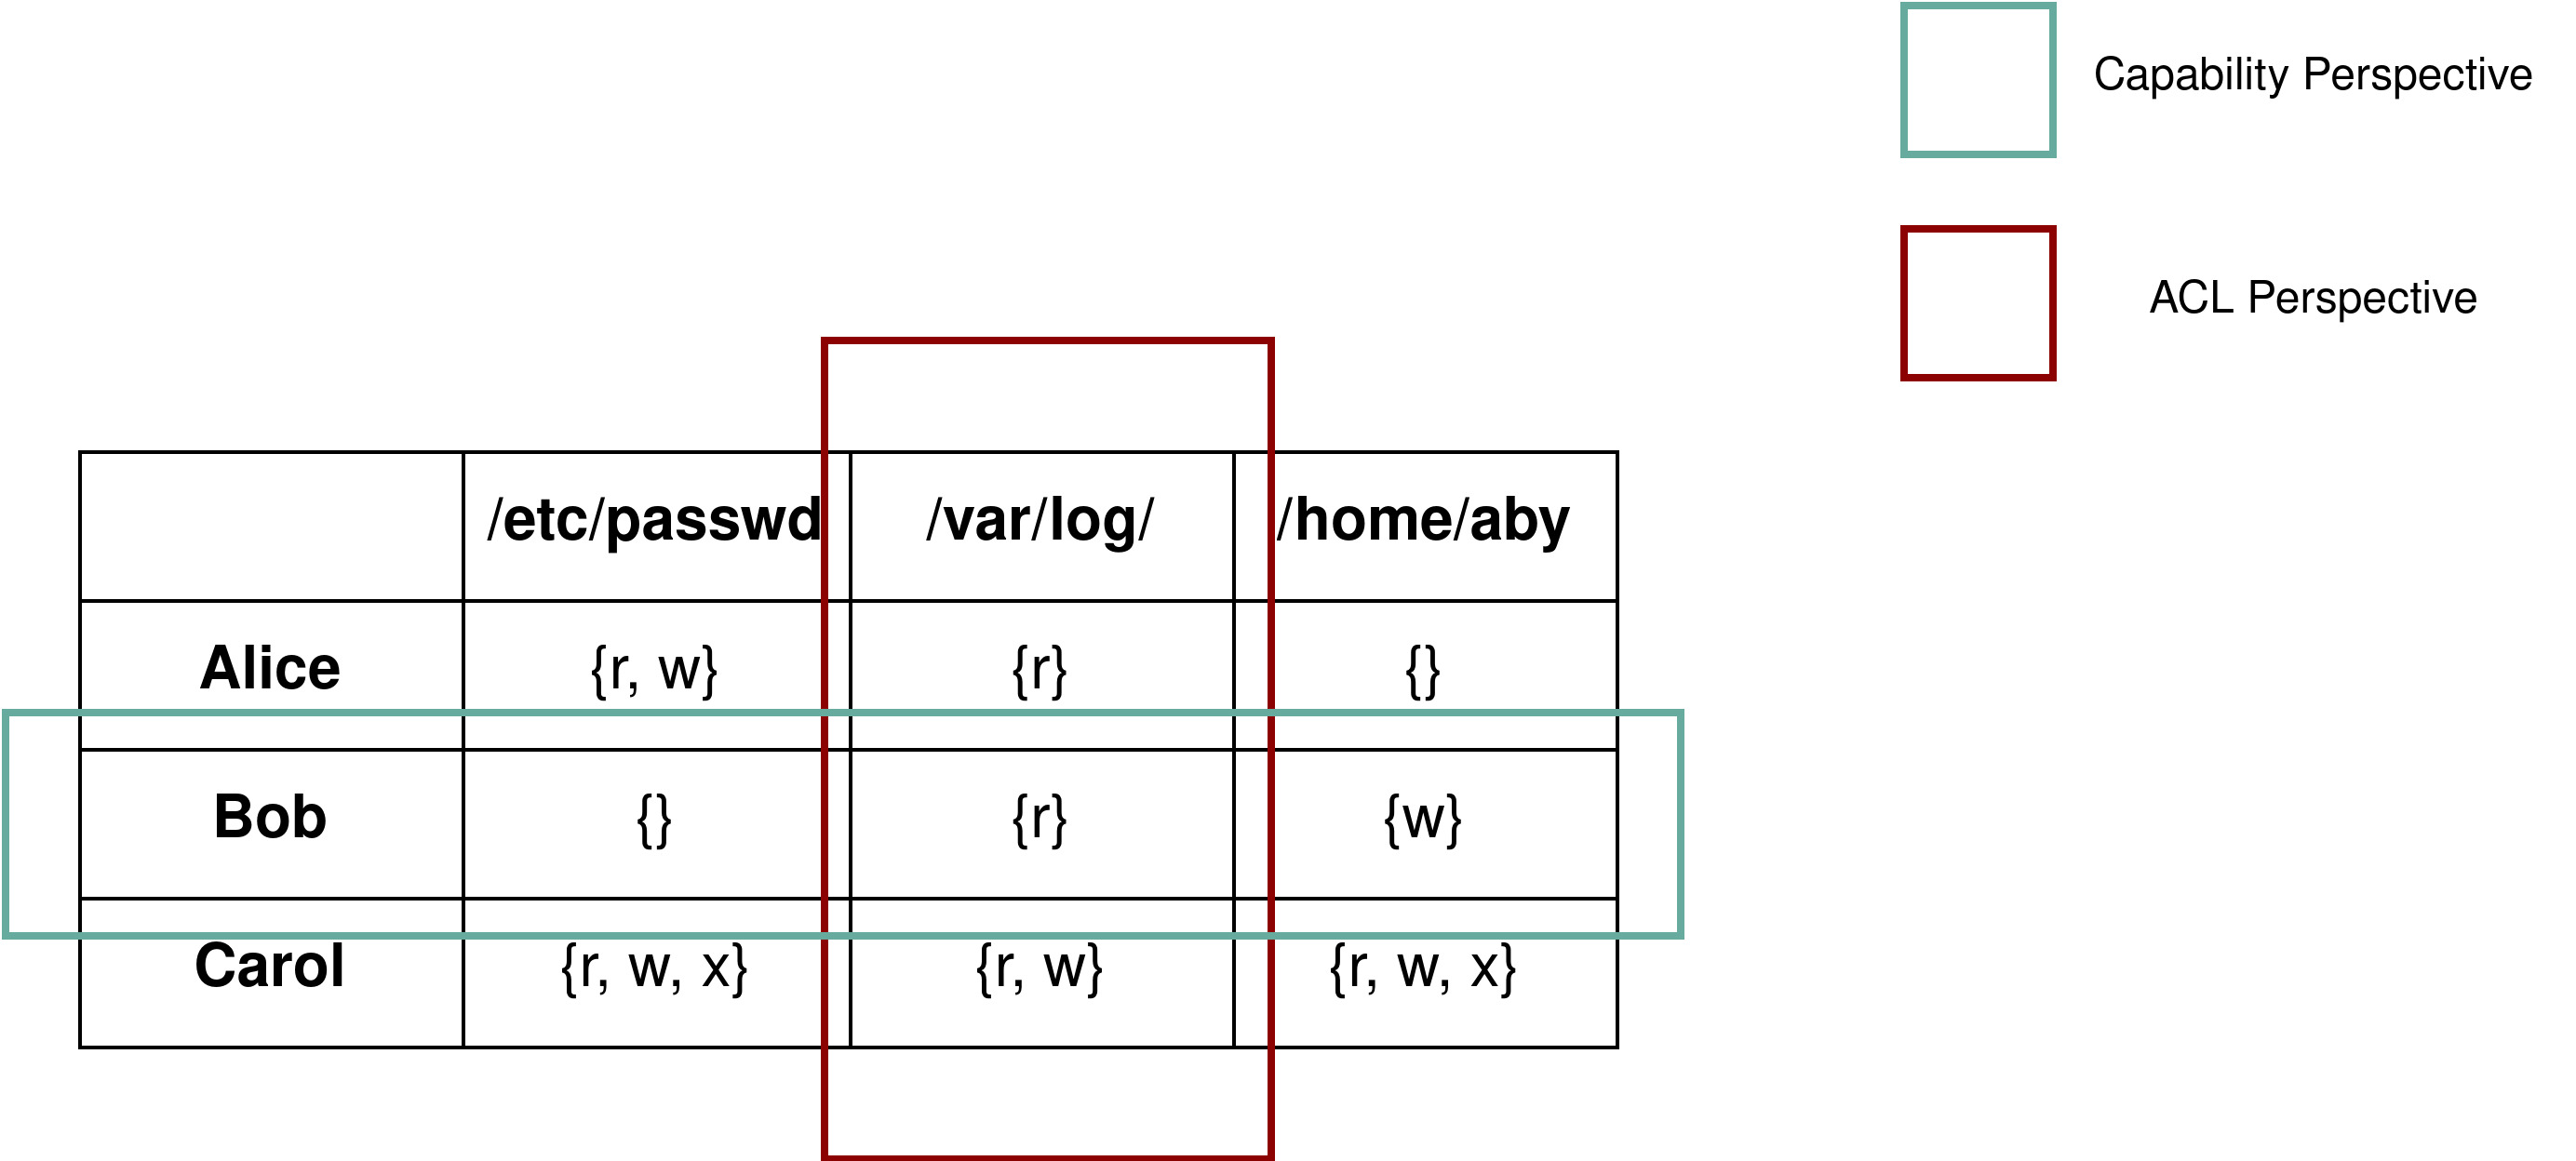
\includegraphics[width=4.0in]{figures/cap_def.jpg}
% \caption{Comparison between ACLs and Capabilities}
% \label{cap_acl}
% \end{figure}

% Here, the authority is defined from a subset of \( {r, w, x} \), which means read, write, and execute on a specific file, respectively. We can see that rows are represented with capabilities for a specific object, and columns are represented as ACLs. Now, this makes a difference in terms of who is bounded to the specific authority (represented with a cell in the table). 

% In ACLs, the resources are bound to the authority, whereas in the capabilities models, it is bound to the specific object. Now, 

\subsection{Capability Patterns: Sealer-Unsealer}

\noindent
According to \cite{millerFinancial}, sealer/unsealer pairs (Figure \ref{fig:sealerUnsealerDef}) can be conceptually viewed as similar to public/private key pairs. They can be used to control rights to access a certain object as follows:
\begin{enumerate}
    \item \textbf{Initialisation} The main program creates the sealer/unsealer pair, and passes it to Alice.
    \item \textbf{Sealing the resource} Alice invokes \texttt{seal} from a sealer object. Internally, \texttt{Sealer} creates a Sealed box, and returns it to Alice. This is represented by steps (1)-(3) in Figure \ref{fig:sealerUnsealerDef}. Considering that Alice only has access to the Sealed Box, she can pass it around without having to worry about others accessing the critical resource.
    \item \textbf{Unsealing the resource} However, Alice must be careful with passing the Unsealer around. If she passes it to another entity (this is acceptable within the design of the language since behavior is defined in trusted code, and not at runtime), they now have the ability to call unseal and gain access to the inner object. This is represented by steps (4)-(6) in Figure \ref{fig:sealerUnsealerDef}. 
\end{enumerate}

This  pattern will be used in the study design of Simple Money, which is given in section \ref{sec:simpleMoney}.

\begin{figure}[htbp]
\centering
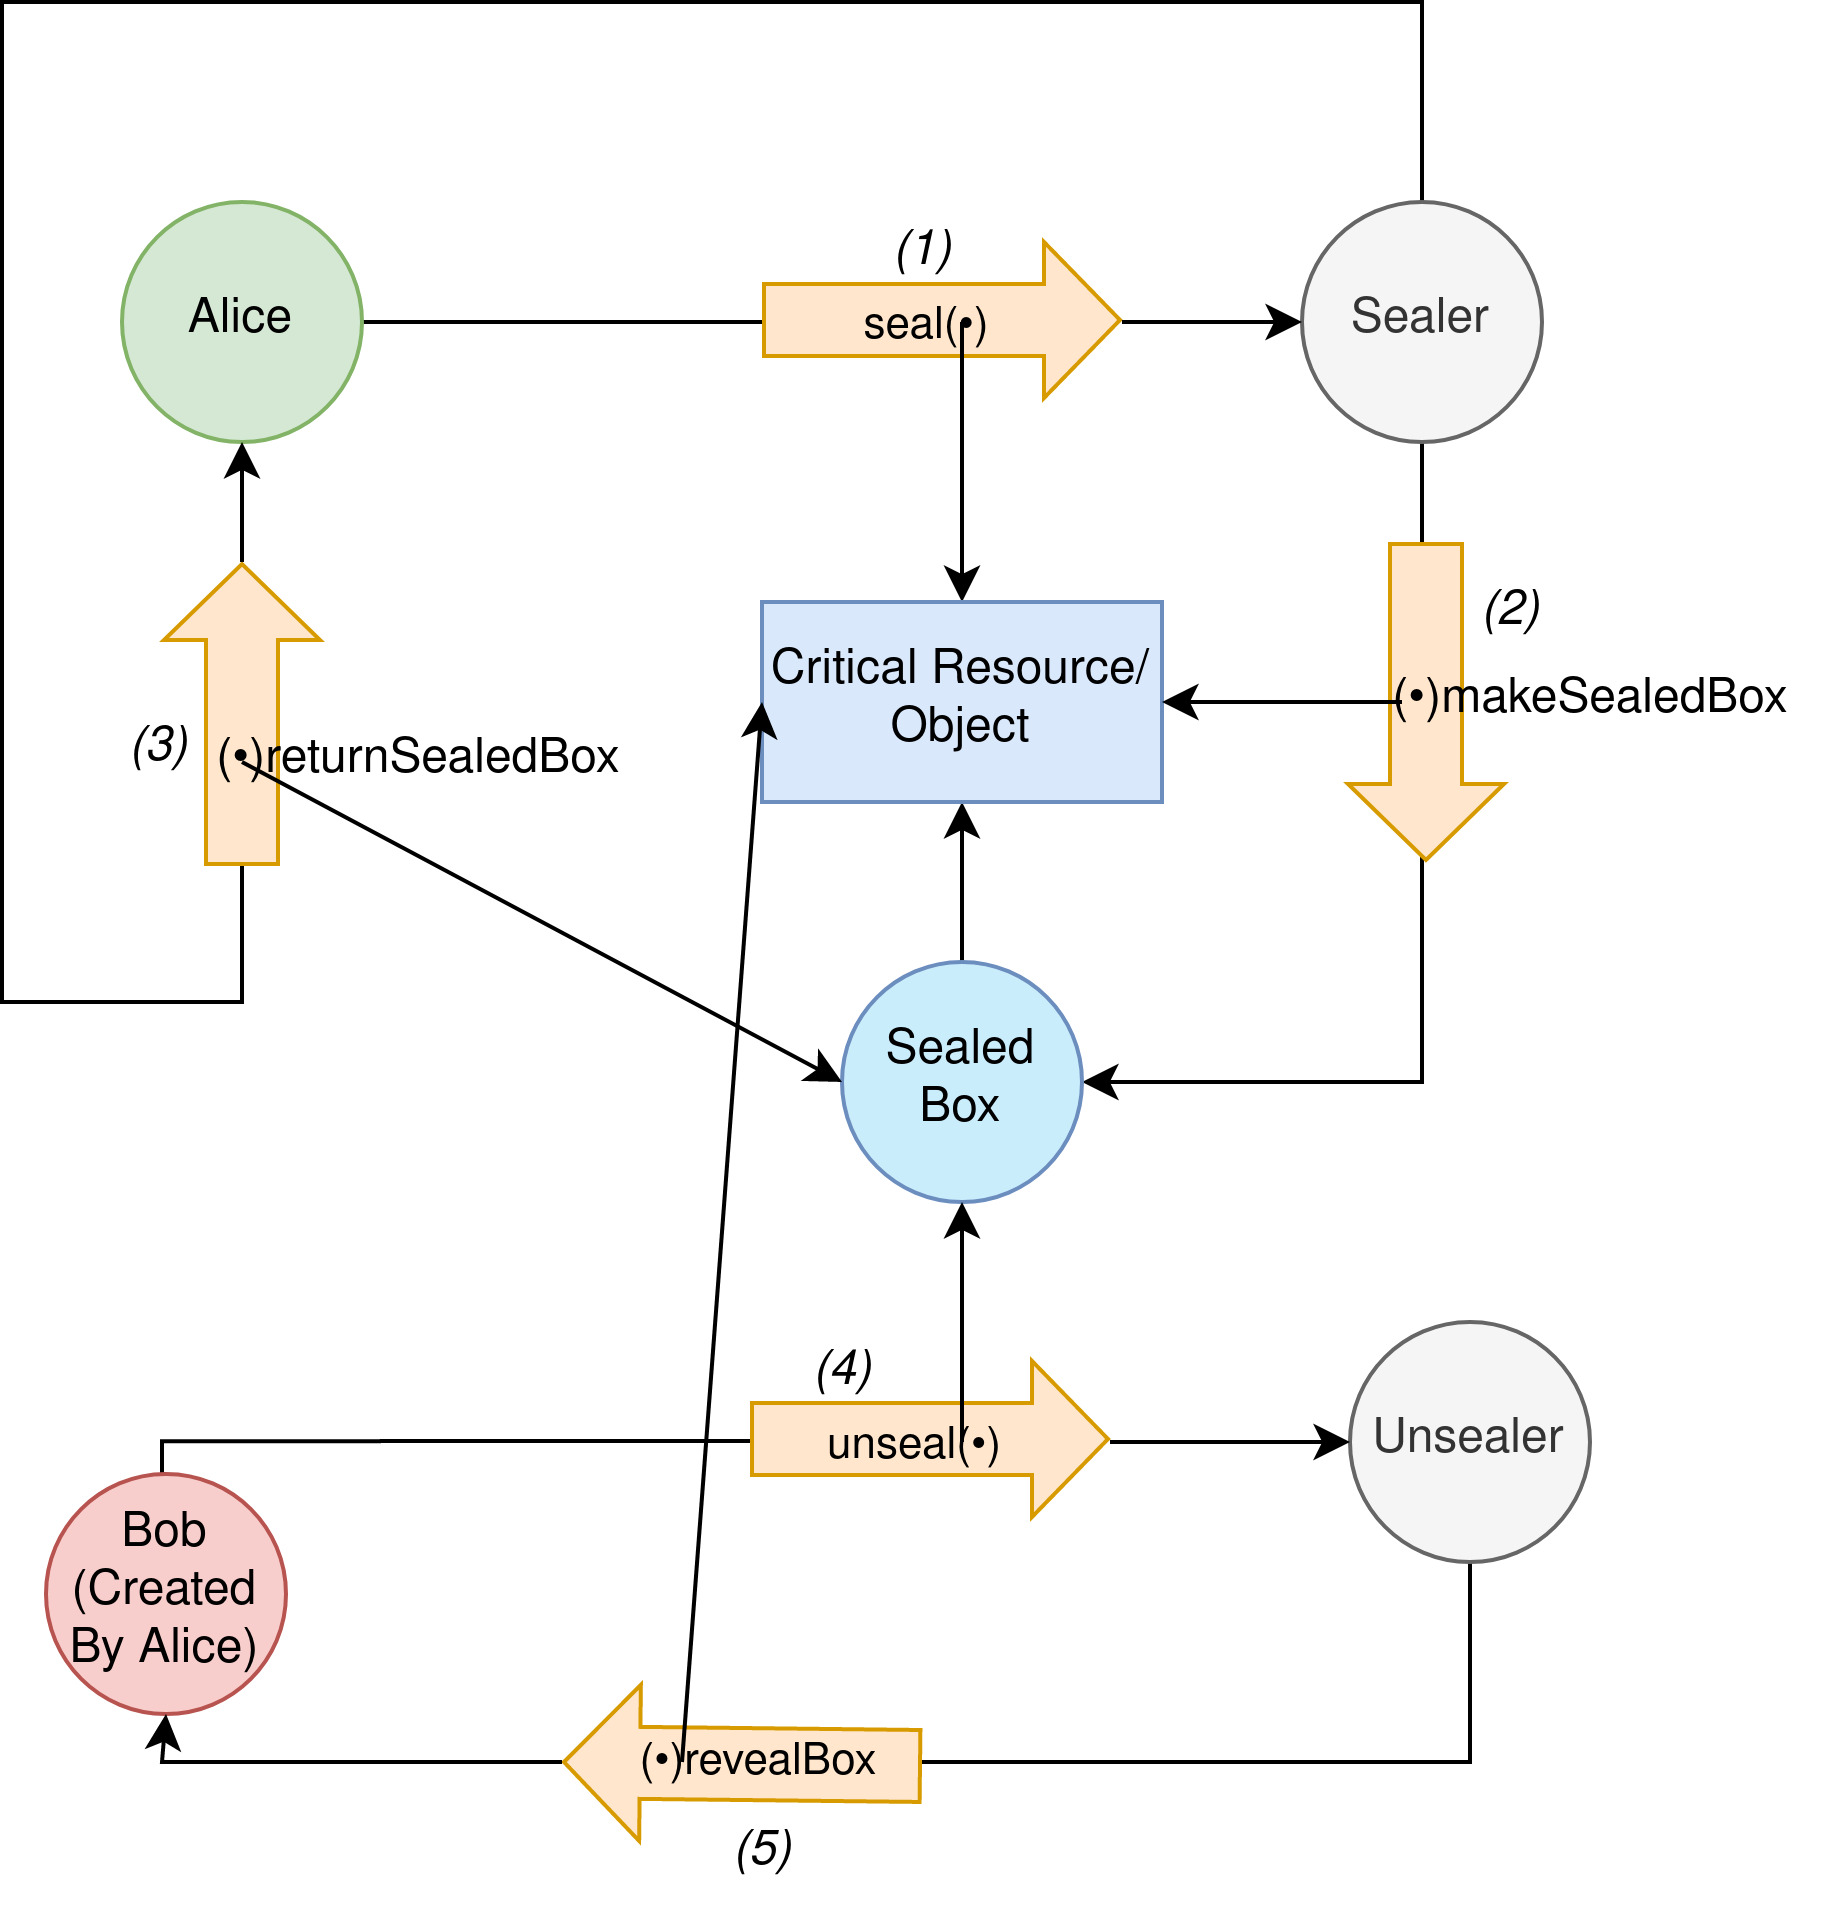
\includegraphics[width=2.5in]{figures/sealerUnsealer_def.jpg}
\caption{Sealer-Unsealer Architecture}
\label{fig:sealerUnsealerDef}
\end{figure}
% \section{Programming Languages}
% \subsubsection{Wyvern}
% \subsubsection{Rust}

\section{Methodology}\label{sec-methodology}

\noindent
To gain insight into the usability of capable and incapable module systems, we set up a qualitative language usability study. For that, we applied for Human Ethics approval from ANU Research Information Enterprise System \cite{aries} for approval. The resulting methodology comprised the following aspects: 

% Recruitment
\noindent
\textbf{Recruitment} Participants were recruited within the School of Computing at the Australian National University. The method of recruitment was to contact potential participants via email or face-to-face interaction. Some of the places include:
\begin{itemize}
    \item Personal/Professional connections
    \item Face-to-face interactions with club members of the Computer Science Student Association (CSSA)
    \item Students completing research in programming languages 
\end{itemize}

In recognition of the participant's time, we renumerated them with a AUD\$20 or AUD\$30 Westfield voucher, depending on availability.



\vspace{-0.5em}
% Participants
\begin{table}[h]
\begin{center}
\begin{tabular}{|c|c|c|c|}
\hline
\textbf{Participant} & \textbf{Background} & \textbf{Programming Experience} & \textbf{Task} \\
\hline
P1 & Parallel Systems   & 5 years & Logger Editor \\
P2 & Systems/Security   & 7 years & Network Pool \\
P3 & Formal Methods     & 3 years & Network Pool \\
P4 & Data Science       & 5-6 years & Simple Money \\
\hline
\end{tabular}
\end{center}
\caption{\label{parDet} Participant Details}
\end{table}
% Years of programming experience
\vspace{-1.5em}
\noindent
\textbf{Participants} Participants at ANU have been chosen because of close proximity to the place where the interviews had to be conducted. To maintain an appropriate level of experience and skills for the pilot study, senior undergraduate/postgraduate students were chosen. The participants should have the necessary background to be able to solve the proposed problem and answer questions during the interview time frame. They had chosen from varied backgrounds to get a more representative study for language designers. Their details are provided in Table \ref{parDet}.

Considering that there are only four participants, the reader may assume a low number of participants is a threat to the validity of the result. However, previous successful studies using thematic analysis have been conducted with only four participants \cite{Huang2023}, and using think-aloud protocol with six participants \cite{whalley2014qualitative}. The papers had the central theme of designing the setup of the study design open-ended to conduct an in-depth analysis of individual studies; and screening tests of the participants. 

% Procedure
% think-aloud programming sessions with semi-structured interviews
\noindent
\textbf{Procedure}  We conducted the study in the format of a semi-structured interview and following the think-aloud protocol. A set of tasks were designed that can be given to either software architects or experienced software engineers that involved designing or extending a small product architecture. 

We use the think-aloud protocol by building on studies done to understand novice programers' strategy who had little experience in programming (\cite{whalley2014qualitative},  \cite{lye2014review}). They partially apply in our case, considering the participants have had no experience in Wyvern, and two out of four participants had prior experience with Rust. However, it should be noted that our pre-screening of participants requires that they have the appropriate level of knowledge in computer science. \cite{whalley2014qualitative} also used narrative analysis, whereas this research project aims to generate results by thematic analysis. \cite{lye2014review} is in the context of developing computational thinking in general; however, our goal is much more specific - to use computational thinking at a higher abstraction level to design modular architectures.

We asked participants to first use a language with support for modules and object capabilities (e.g. Wyvern), and then use a more traditional language with external capability libraries (e.g. Rust/Java) to design the same architecture. Documentation links related to standard capability libraries in Rust (\cite{libcaprust}, \cite{libcapdirrust}, \cite{librust}) were provided as starting points. After this, we asked them to break the security of the written program itself for any/both languages, to reveal potentially overlooked vulnerabilities. 

Finally, we asked post-interview questions consisting of a survey (details of questions are provided in appendix \ref{sec-appendix}). The total length of each study was 90 minutes, with each section having a rough outline of the overall time distribution:
\begin{enumerate}
    \item \textbf{Rust and Wyvern Implementation} (60 mins)
    \item \textbf{Trying to break security of the Program} (20 mins)
    \item \textbf{Post-study survey} (10 mins)
\end{enumerate}

Occasionally, we took notes regarding how the discussion went, and marked points of potential interest to double down on when conducting thematic analysis. If a student was stuck on a part, we asked them to explain their thinking process using the think-aloud protocol.

% Data collection
 
\noindent
\textbf{Data Collection} The data being collected was personal information about the interviewee's previous experience in software development, domain of expertise, and current role. During the interview, the information being collected was: (a) Screen recording of the desktop environment (b) Audio transcript (c) A survey at the end of the interview (full-list of questions provided in appendix \ref{sec-appendix}). \label{survey} \label{sec:dataCollection}


% Analysis
\noindent
\textbf{Analysis} Thematic analsysis is now commonly used in the programming languages research community for various use cases, such as highlighting key challenges in language design \cite{Coblenz2023} and its tooling, and debugging \cite{Huang2023}. The main goals of the referenced studies also apply to our overarching topic of determining the suitability of a language for a given task.

We conducted a thematic analysis of the code, audio-recorded interview and the post-interview survey to derive potential hypotheses. The analysis was conducted by keeping two major themes in mind: The usability of both languages and any Security Vulnerabilities that could have arisen. In our case, the procedure would look like the following: If one is taking an audio-recorded interview, the initial step is transcribing the sampled data. Our data sources also consist of screen sharing, so it is essential to mark points of interest (errors in code, completion, etc.) as well. The next step is to look for recurring themes from each interview. We follow this up in Section \ref{sec-results}.

\section{Study Design}\label{sec-content}
\noindent
The overall study consists of three parts. In each part, we ask participants to implement specific parts of the architecture using capabilities via external libraries or via module systems in languages. Each part was designed to primarily test one of the facets of the overall goal (usability, extensibility, and security); however, all facets were considered in the analysis of each part.

Each study part was divided into three steps for participants - designing the initial architecture, finding vulnerabilities, and the post-study survey.\footnote{Code templates for the studies are available at \url{https://github.com/abhaasgoyal/module-systems/tree/plateau-2024}} 

\subsection{Logger Editor} \label{sec:loggerEditor}
\begin{figure}[htbp]
\centering
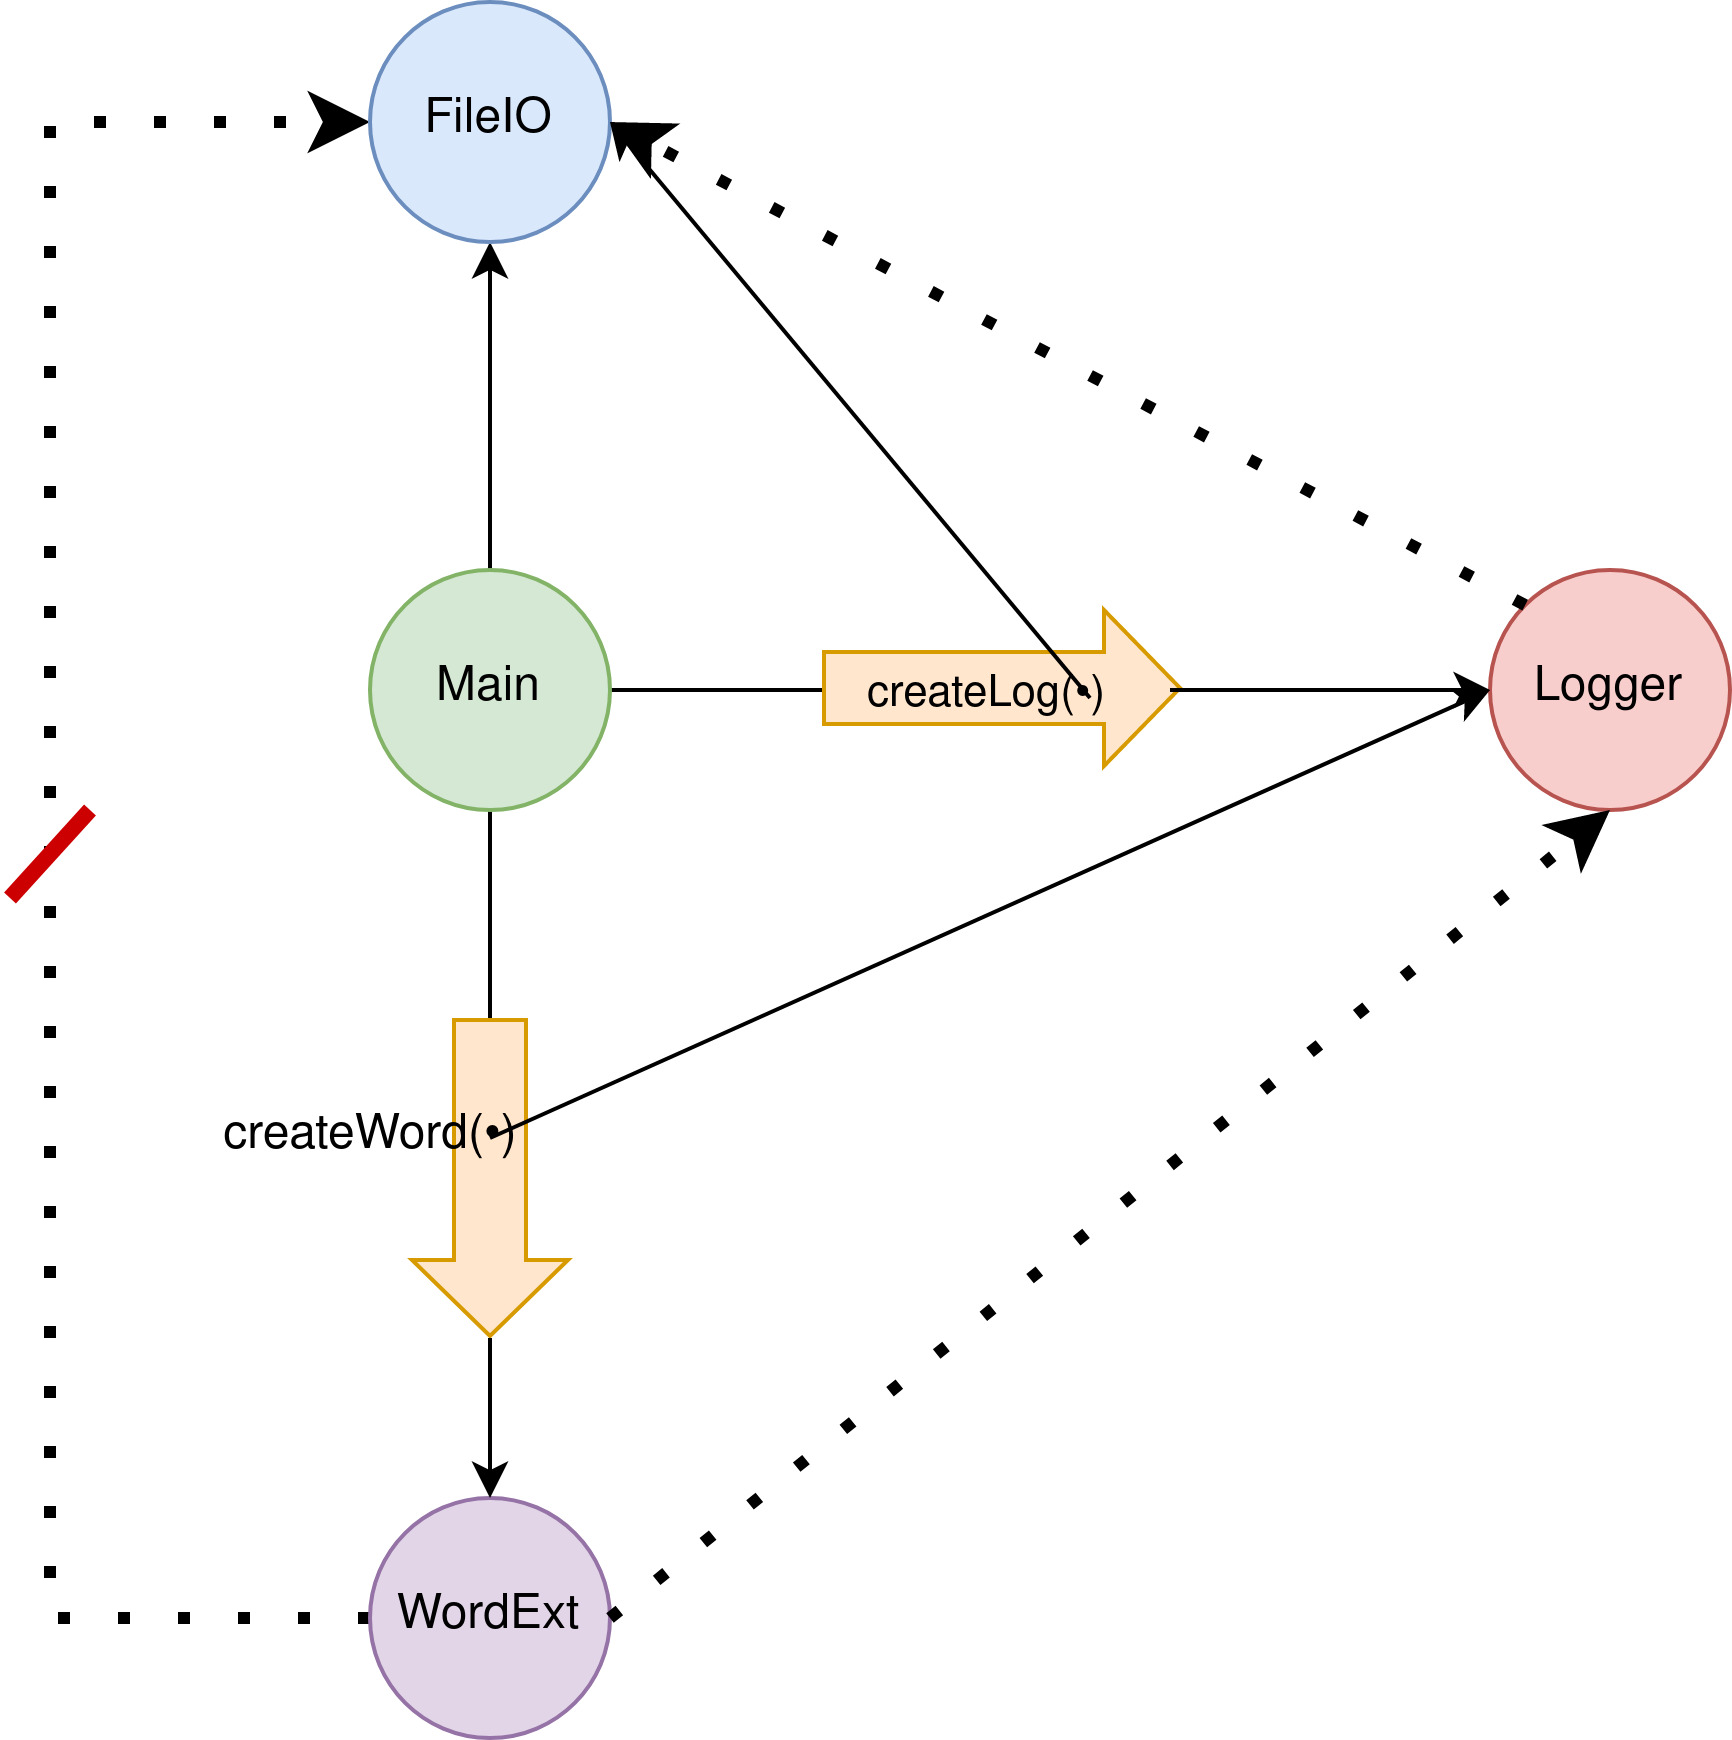
\includegraphics[width=2.2in]{figures/Ambient_logger.jpg}
\caption{Logger Editor}
\label{loggerEditor}
\end{figure}
\noindent
\textbf{Purpose} To assess the security of participant code, ensuring that authority is non-transitive.

% https://drops.dagstuhl.de/opus/volltexte/2017/7270/pdf/LIPIcs-ECOOP-2017-20.pdf
\noindent
\textbf{Background} In figure \ref{loggerEditor}, the \texttt{Main} application has a \texttt{Logger} module that it can trust. The logger module has access to \texttt{FileIO}, providing it the authority to read/write to files. However, there also exists an extension named \texttt{wordCloud} module, which needs to utilize the \texttt{Logger} library to read/write to a place that only \texttt{Logger} can allow. Here, \texttt{Main} passes \texttt{Logger} when creating \texttt{wordCloud}. The goal of the user is to design \texttt{Logger} in such a way that \texttt{WordExt} does not have access to the underlying module \texttt{fileIO} and, in the process, escalate its privilege.

% \noindent
% \textbf{Additional Specifications}
% The following requirements need to be satisfied when designing the logger architecture for specific languages:
% \begin{itemize}
%     \item The name of the log file should be \texttt{log.txt}
%     \item The directory containing the file would depend on the language as follows:
%     \begin{itemize}
%         \item \textbf{Rust} Stored in the env variable \texttt{\$DATA\_DIR} (since Rust's capability library provides inbuilt support for writing directly to that folder)
%         \item \textbf{Wyvern} Stored within the same folder as the program
%     \end{itemize}
% \end{itemize}
\subsubsection{Instructions}
\noindent
\textbf{Rust Implementation}
The implementation in Rust was based on the \texttt{cap-std} module \cite{rustCap}. The implementation should contain the functionalities for the following (note that one can change the function names in the Extension depending on how the Logger is structured): 

\begin{itemize}
    \item \mintinline{Rust}{create_logger(logFile: String)} - A constructor which returns a new logger object with the name logFile
    \item \mintinline{rust}{logFile.append_to_log(entry : String)} - Append a new entry to the logFile
\end{itemize}


Given a possibly malicious \mintinline{Rust}{extension.rs}, design the corresponding Logger module with capability library in Rust.

\noindent
\textbf{Wyvern Implementation} The extension library is \texttt{wordCloud}, and the users need to design the logger library from scratch with the \texttt{appendLog} function. Since capabilities are hierarchical here, the users were given a more open-ended specification of the parameters of the logger library; the solution is that the underlying \texttt{fileIO} system resource is passed exclusively to the logger from Main.

There was no developer-friendly documentation available for Wyvern's standard I/O library, so we provided the implementation, hoping that it will act as self-documenting code. The required method definitions for \texttt{fileIO} are provided in listing \ref{code:fileIOwyv}.

\noindent
\textbf{Trying to Break security} Upon completing the corresponding functions, users were asked to find a way to bypass the restriction of accessing \texttt{fileIO} in the corresponding programs, while only modifying \texttt{Extension.rs} (for Rust) and \texttt{wordCloud} module (for Wyvern).

\subsection{Network Pool}\label{sec:networkPool}

\begin{figure}[htbp]
\centering
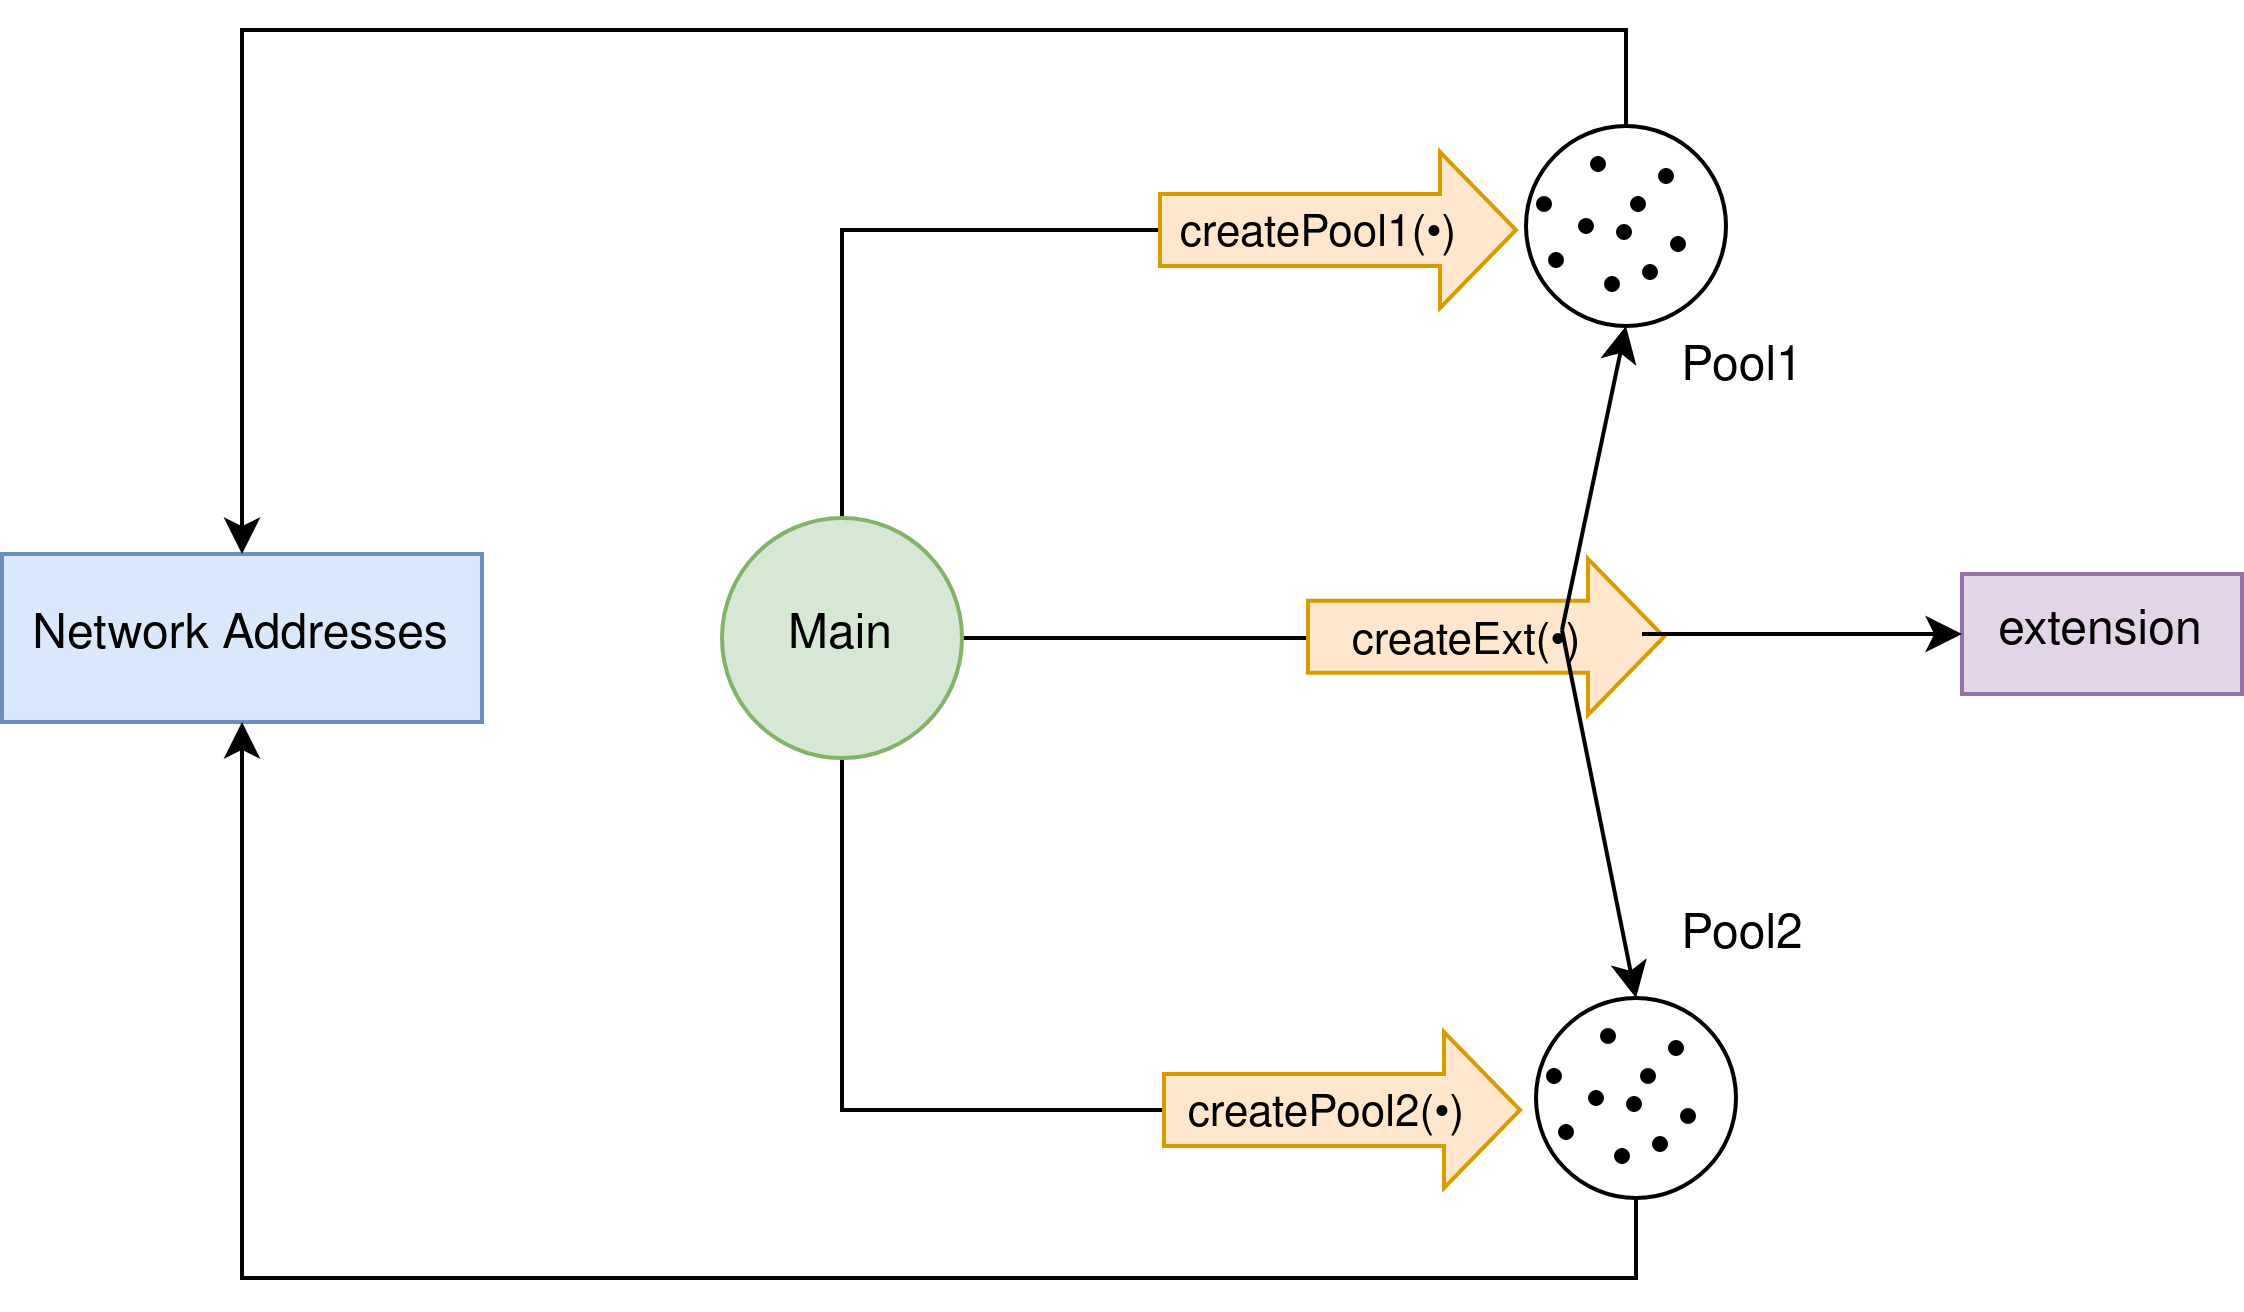
\includegraphics[width=2.8in]{figures/network.jpg}
\caption{Network Pool (A dotted circle is the capability to connect to a specific device)}
\label{fig:network}
\end{figure}

\noindent
\textbf{Purpose} To assess the ease of developing appropriate implementations from the specification. A high degree of freedom should be provided in how to design programs.

\noindent
\textbf{Goal} Firewalls are essential to control incoming and outgoing network traffic. The user has to implement a basic firewall by making two kinds of network pools that allow an untrusted extension to use the network in limited ways. The extension promises to only connect to the website \texttt{example.com}. The architecture can be represented with figure \ref{fig:network}. There are two types of pools used in the Extension. The pools should limit the extension to the following authorities, respectively:

\begin{itemize}
    \item \textbf{TCP-Port} Only allow connections to an IP address of \texttt{93.184.216.14} using a TCP port (0-65535). For Wyvern, it can be assumed that the IP address is a string of fixed length i.e.\ it has a length of 15. For example, \texttt{192.68.1.1} is represented as \texttt{192.068.001.001}
    \item \textbf{Net-Port} Only allow connections to a small range of IP addresses (but with any port allowed). The last 8 bits of the IP addresses should be in the range \texttt{93.184.216.<0-255>}
\end{itemize}

\subsubsection{Instructions}
\noindent
\textbf{Rust Implementation} Within \texttt{pool\_auth.rs}, create the respective network pools by looking at the necessary documentation. Then, call in the Extension by passing in the Pools with the required IP address and HTTP port in both cases as the input. In this case, the necessary documentation was regarding Network Pools implementation  in capability standard library of Rust \cite{libcaprustpool}.
 

\noindent
\textbf{Wyvern Implementation} The \texttt{makePool} module should have 4 input parameters - \texttt{startIp}, \texttt{endIp}, \texttt{startPort}, and \texttt{endPort}.
Then, come up with an abstraction of functions for Net-Port and TCP-Port, which call \texttt{makePool}. This should be within the main function.
Finally, the function \texttt{connect(addr, port)} should consist of a guard which checks whether the \texttt{addr} and \texttt{port} are within the acceptable range, and connects if the check succeeds.

\noindent
\textbf{Trying to Break security} This exercise was similar to the Logger-Editor design, but now considering multiple capabilities that are passed to the Extension. Upon completing the corresponding functions, try to break the security of the filesystem in the corresponding programs by modifying only \texttt{Extension.rs} (for Rust) and the \texttt{cloud} module (for Wyvern).

\subsection{Simple Money} \label{sec:simpleMoney}
\noindent
Note: The design was motivated by the simple money example \cite{millerFinancial}.

\begin{figure}[htbp]
\centering
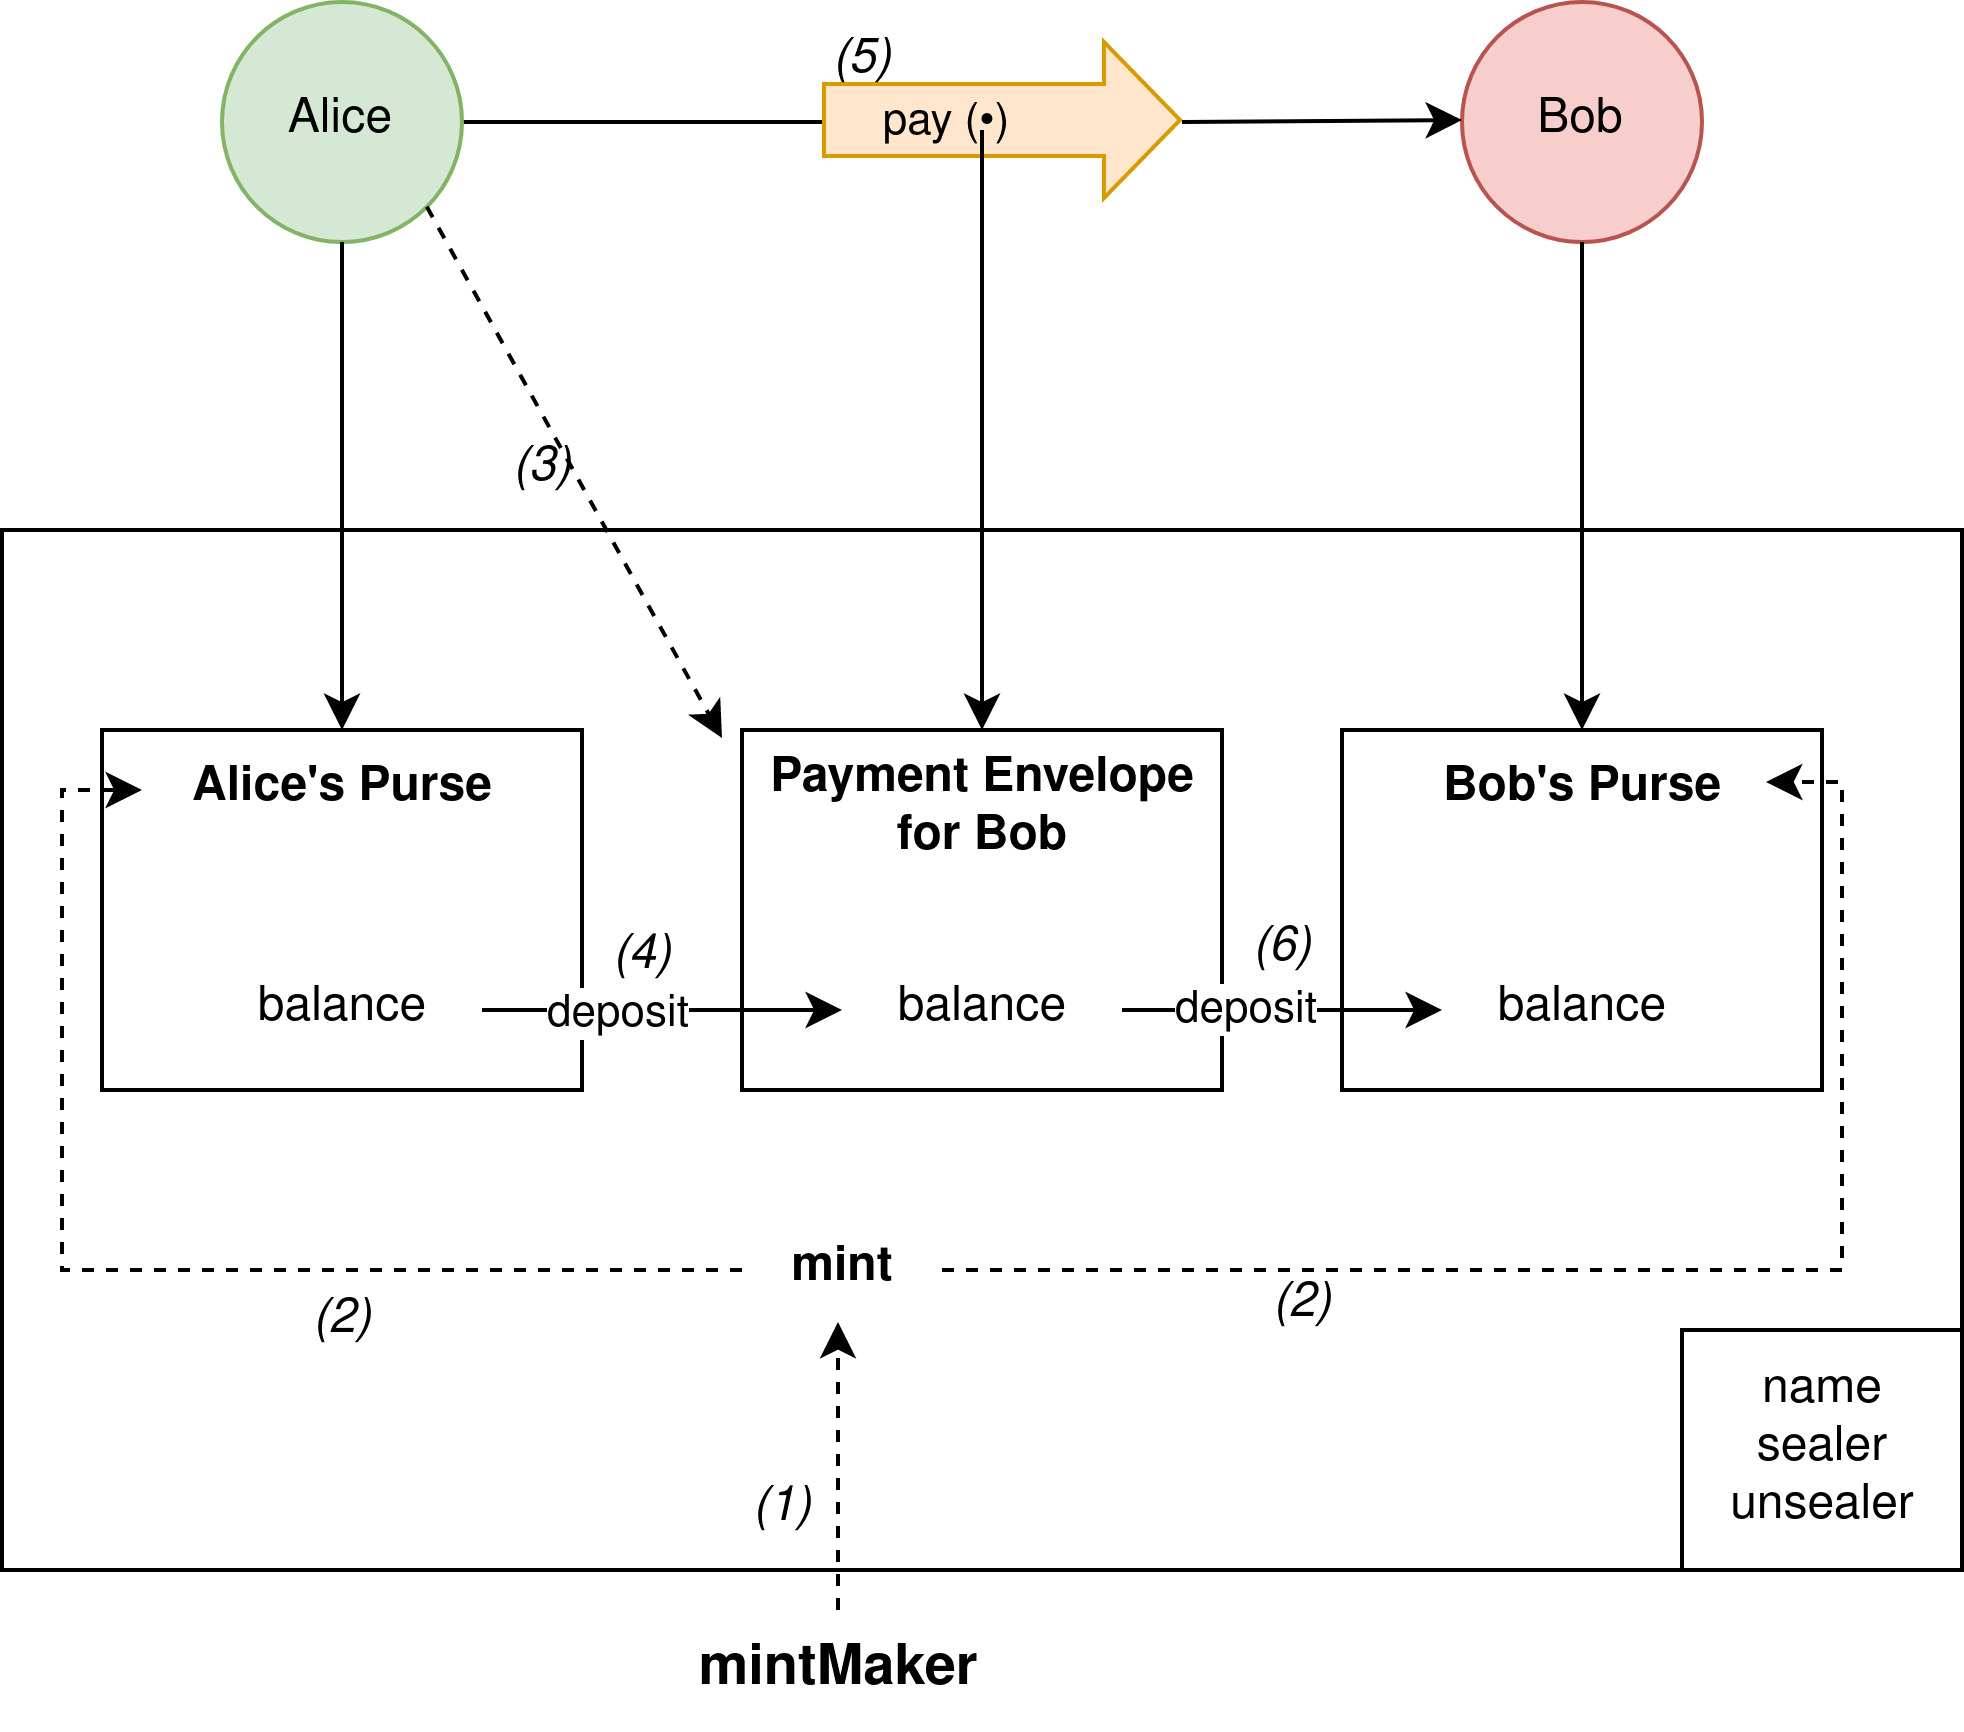
\includegraphics[width=2.6in]{figures/simpleMoney.jpg}
\caption{\label{fig:simpleMoney} Simple Money}
\end{figure}

\noindent
\textbf{Goal} Extensibility of adding code to existing codebases.

\noindent
\textbf{Background} Given a money minter and two purses A and B, design a transaction where user A can securely send money to user B, using the capability pattern of sealer-unsealer. 

\noindent
\textbf{Architecture}
The architecture (figure \ref{fig:simpleMoney}) consisted of the main entity \texttt{mintMaker}, making the \texttt{Mint} Object, representing a new currency. It has a fixed amount of total balance. It employs the Factory Pattern to further create two \texttt{Purse} objects, Alice and Bob, which it can initialize with a certain balance. This is implemented in steps (1)-(2). Now, the question is whether Alice can pay some of her money to Bob while conserving the total currency. Some of the goals the architecture needs to achieve \cite{millerFinancial} are:
\begin{itemize}
    \item (T1) Only someone with the mint has the power to change the total balance of that currency
    \item (T2) \texttt{Purse A} cannot change the balance of \texttt{Purse B}
    \item (T3) Balances should always be positive
    \item (T4) If a successful deposit gets reported, Alice should be guaranteed that the deposit was made to the other wallet
\end{itemize}

\subsubsection{Instructions}
\noindent
The participant is given implementations of the Sealer and Unsealer primitives, as well as the Mint object (steps (1)-(2) in the diagram). The user tasks for both languages were to securely transfer money via an intermediate Purse Object with the Sealer-Unsealer pattern. The purse should have the following methods:
\begin{enumerate}
    \item \mintinline{rust}{purse.getBalance(): Int} - Get the current balance in the purse  
    \item \mintinline{rust}{sprout(): Purse} - Create a new empty purse 
    \item \mintinline{rust}{getDecr(): SealedBox[Int -> void]} - Get a sealed version of \texttt{decr}. A hint was provided that should be used to validate (T4) during a \texttt{deposit} to Bob's purse. \texttt{decr} is a function that subtracts the balance in the current Purse
    \item \mintinline{rust}{dst.deposit(amount:Int,src:Purse):void} - Securely transmits money from one wallet to another
    \item \mintinline{rust}{print():void} - (Optional) Print debugging information
\end{enumerate}

The programmer's expected steps are to understand the respective codebase and extend the program's functionality. Instructions were the same for Wyvern and Rust implementation, with slightly different filenames. They were to implement the architecture above and then come up with potential vulnerabilities in their implementation.
\section{Results}\label{sec-results}

% The scope of our results lies in validating these in future research.   
\noindent
After conducting the study with four participants, we now construct a thematic analysis and derive hypotheses for each research question. 

\subsection{RQ1: Usability of capabilities in the language vs. library}

% Mean solving time for all 4 participants for Rust and Wyvern. However, P1 mentioned at the end of the survey that switching up the order would be good.
% Answer to survey questions - documentation for Wyvern in general, like rust libraries, influenced what they had to do

\subsubsection{Understandability of existing code and Extensibility}

% In particular, how could the \texttt{dyn} keyword be used for returning traits (when used with the \texttt{struct Box}?
\noindent
(P4) mentioned that understanding the code for Simple Money was highly complicated in Rust, even though they had past experience. In particular, it was related to \texttt{dyn} keyword and its use in traits. This proved to be much easier in Wyvern; however, it may be because Wyvern's implementation matches better with the original problem in terms of objects. Rust's implementation of Simple Money also had all three objects for building objects and their behavior: \texttt{trait}, \texttt{struct}, and \texttt{impl}, which in general, caused a higher cognitive load for the users. This confused the participant as to how different modules were interacting. Another major conceptual hurdle three participants found in Rust  was \texttt{.unwrap()} vs \texttt{?} operator (i.e.\ the \texttt{Option} vs \texttt{Result} type).

In comparison, most concepts in Wyvern came more easily to participants. An example of this would be \texttt{var} vs.\ \texttt{val}. (P2, P4) mentioned they were easy to understand and helped them gain quicker results in Wyvern's implementation. However, there were some concepts in Wyvern that participants had difficulty understanding. A major one was the difference between \texttt{module def} and using plain \texttt{module} when defining abstractions. For \texttt{module def}, most participants were provided with the analogy of the parameters as constructors (data members) along with function definitions. However, (P1) raised an interesting question on \texttt{wordCloud}, where both \texttt{WordFactory.Word} and \texttt{WordFactory} types had been passed as parameters. They asked why both needed to be passed when only \texttt{Word} was needed in the implementation function. Here, the capability to access a value of type \texttt{WordFactory.Word} itself depends on whether we have the existing capability for \texttt{WordFactory} - thus following the rule of no ambient authority. Here, the Main module has to pass both the top-level capability object and sub-capability object to different modules. This could potentially lead to many parameters in module definitions in large systems, which can be considered as a case of \textit{\textbf{overhead}} of using capabilities.

\subsubsection{Writing Syntax} 
\noindent
One of the hurdles faced by participants was that they needed to learn the language syntax better, so the process of writing up the correct syntax could have been faster for both languages. Even though tutorials were designed for each language to implement the specific question to improve productivity, they were limited in scope due to the time constraints of the study itself (we acknowledge this as a limitation of the study design). Although the intention of the study was designed for participants with a general computer science background, having some pre-reading on the documentation of the specific languages before the interview would save significant time and help with more complex studies. This could be achieved with a pre-survey on those specific languages before recruiting.

(P1, P3) felt that a lot of the code in Rust was boilerplate in terms of using appropriate type definitions. This was due to Rust's complex set of borrowing rules. For example, (P1)'s implementation of the logger module's had to change the type of extension to mutable as well (since they structured their logger with the file reference instead of location, and \text{File} is mutable in \texttt{cap-std}. In comparison, users liked that they had to write less code in Wyvern without sacrificing stability. 

Finally, users sometimes found it helpful to have code completion hints in Rust, of which none exist in Wyvern. However, participants faced no significant problems in terms of the time taken to write the program and complete the study on time. 

\subsubsection{Errors and Debugging}
% 4. Documentation a lack of documentation on Wyvern, which was not provided in the tutorial (such as the Option type for P4) stdlib (other than going to the source code itself)

\noindent
\textbf{Rust} Most of the participants found Rust's error messages to be helpful in figuring out bugs, but only once they understood the specific concept. A participant even mentioned that the error messages popping up and fixing them helped the participant learn the language in a short period of time. However, the author would like to be cautious about being totally dependent on errors generated by the compiler. For example, (P2) faced an error in Rust, which suggested that the error was related to invalid types; however, the actual error was that they had missed a semicolon (;) in the previous line. This simple error, with an unrelated message, took a lot of time for the participant to debug.

\noindent
\textbf{Wyvern} All participants noted that Wyvern was highly sensitive to bugs in lexical analysis and parsing, which made it hard to debug the exact cause of the issue. This has to do with Wyvern being in its initial stages of development. However, they used line numbers in the error message to estimate where the bug resided and tried to change the code on a trial-and-error basis. In cases where the participant could not solve the issue, we acted as the manual compiler and helped the participant fix errors in this case. It is also essential to see that Rust's documentation is more comprehensive than Wyvern's, with answers to specific questions on websites like StackOverflow. Hence, if the participant was stuck for a long in a problem with Wyvern, we acted as the StackOverflow entity in that scenario. One of the most common errors faced by participants was mismatching function/type definitions in Wyvern's specification and implementation. For example, (P3) realized that they needed to change the following module definition when creating connect: % 44:00

\begin{minted}{rust}
// Original code
module def poolMaker(startIp: String, endIp: String, startPort: Int, endPort: Int): PoolMaker
def connect(address: String, port: String): String 
// Proposed change
def connect(address: String, port: Int): String
\end{minted}

\noindent
However, this change requires changes in \texttt{PoolMaker} module as well:
\begin{minted}{rust}
resource type PoolMaker
   def connect(address: String, port: Int): String
\end{minted}

\noindent
From the points above, we arrive at a hypothesis on the usability of capable and incapable languages: 

\begin{hyp}[Usability]
With fewer keywords in the language specification, Wyvern is easier to learn in terms of syntax. Furthermore, compared to Rust, it provides better structure in terms of reducing cognitive overhead when designing programs. However, there is a desire for (a) minimizing the capability overhead on expressing capabilities in terms of language syntax and (b) improving the debugging, documentation, and code completion, which accounts for factors in the lack of usability for the language.
\end{hyp}

\subsection{RQ2: Analysing Security of Capability-Designed Languages}
\noindent
In total, two types of vulnerabilities were found among the participants:
\begin{itemize}
    \item One of the participants found the vulnerability in Network Pool (\ref{sec:networkPool}) in Rust. They circumvented the need to use a specific Pool object by importing \texttt{cap-std} within the extension. When the extension function is called, they can now create a new Network Pool with \textbf{any} privilege and connect to the network from there. There are no checks by the network connector whether the extension module itself had the capability to access specific addresses. This could also be carried on for the Logger Editor Example in terms of file systems. The participant could not think of a solution in the time frame. Now, this raises an interesting point. The Main module has to look for all types of imports within the whole codebase. Based on that, trust the extension. However, this is not feasible in large software, where developers interact via function API documentation. This problem was not faced in Wyvern, which could provide a potential use case for using capability-based language design.
    \item (P4) found a vulnerability in creating additional Minters in both Rust and Wyvern; however could not break the security of a single transaction. As such, both architectures were equally secure in terms of implementation. 
\end{itemize}

\noindent
Thus, we reach the following hypothesis on the security of capable and incapable module systems: 

\begin{hyp}[Security]
It was seen that capabilities ensured additional levels of security compared to other modern programming languages in the context of trusting the API definition. However, to see wider adoption from language designers, more work is required to classify more security bugs that only capabilities can solve. 
\end{hyp}
\subsection{Threats to Validity}
\noindent
It should be noted that the hypotheses state are derived from preliminary results. Therefore, a more thorough study is required to validate them, which would address the following threats to validity:

\noindent
\textbf{Participants} All recruited participants were from the same institution, all of whom were recent graduates or undergraduates. We attempted to resolve this by having a brief pre-screening with the participants. We asked them general questions regarding computer science concepts, which would ensure that participants had the appropriate knowledge to implement concepts in the study. However, it should be seen that the participants did not have much experience with designing software architecture in the industry, which would lead to more security bugs in the underlying code and a limitation in detecting potential bugs. 

\noindent
\textbf{Prior Experience} Considering that Wyvern is currently under research and Rust is an upcoming language in the mainstream, not many people have had prior programming experience in the specific languages. This could have made programming slower.

\noindent
\textbf{Study Procedure}: Considering that we were asking the same subjects to break their own code, most of them (except one participant) could not think of a way on how to do this. The order in which these languages were studied is also important since participants already had a fair idea of the problem when implementing it in a different language. This could be one of the reasons why participants found it easier to code in Wyvern than in Rust. More anecdotal evidence conducted in a suitable design would answer this question. For this, a potential alternative study design is to give participants another participant's code to break the security (similar to pen testing in companies) since finding vulnerabilities from a different solution is from a different experience. % Citations?
\section{Concluding Remarks}\label{sec-conclusion}

\subsection{Conclusion}

\noindent
We conducted a comparative study of traditional versus capability-based module systems by interviewing four upper-level undergraduate students. In doing so, we identified two main hypotheses relating to the usability and security of programs in capability-based languages to help programmers be productive and motivate further work in researching further secure systems. % to improve

We hope these hypotheses will improve the understanding of reasons to design secure programming languages via capability-based language systems. Furthermore, if principles from the study are used to provide better tooling for existing capability-based languages, we hope that it will have broad benefits in terms of writing better software in terms of programmer productivity, security, and extensibility.

\subsection{Future Work}

\noindent
Current results show that we have only scratched the surface in this problem domain. Further avenues for research mainly include improving the design of the study based on the following:

\noindent
\textbf{Larger target audience} Preferably working professionals who are domain experts with at least one of the programming languages being surveyed. We found that our study needed quantitative analysis and collect more anecdotal evidence to support our claims. The current sample size is small for doing any of the two. This would also help us use more complex software design problems during interviews.  

% https://doi.org/10.14236%2Fewic%2FHCI2008.9
\noindent
\textbf{Including more modern programming languages} For a more comprehensive comparison and seeing what features are needed in capability-based designed languages to make it more usable for general programmers without sacrificing security.

\noindent
\textbf{Finding more Security Vulnerabilities} The study designs should be based on existing CVE vulnerabilities. Vulnerabilities classified in CVEs are based on large-scale software, where decisions are made on an architectural level. We can design studies about employing capabilities patterns on larger systems to achieve this.

% \textbf{Grounded Theory Study} - Validating/coming up with hypothesis. - Maybe thematic analysis is not enough here

% inference for SML

\printbibliography 

\appendix
\section{Appendix}\label{sec-appendix}

\subsection{Post-study survery questions for Study Designs}
\begin{enumerate}
    \item How useful do you think capabilities are?
    \item How much did you like working on Wyvern? 
    \item How much did you like working on Rust?
    \item How much did you think you understand the concept of capabilities?
    \item What are some things that you would have wanted to improve in the survey if you had the chance to do it all over again? 
\end{enumerate}

\subsection{FileIO in Wyvern}

\begin{minted}{rust}
import fileSystem.BoundedReader
import fileSystem.Writer
import fileSystem.RandomAccessFile
import fileSystem.BinaryReader
import fileSystem.BinaryWriter
resource type File
    effect Read
    effect Write
    effect Append
    def makeReader(): {} BoundedReader
    def makeWriter(): {} Writer[{this.Write, this.Append}]
    def makeAppender(): {} Writer[{this.Append}]
    def makeBinaryReader(): {} BinaryReader
    def makeBinaryWriter(): {} BinaryWriter
    def makeRandomAccessFile(mode : String): {} RandomAccessFile
\end{minted}
\label{code:fileIOwyv}

\subsection{Post-Study Survey}

\begin{figure}[htbp]
\centering
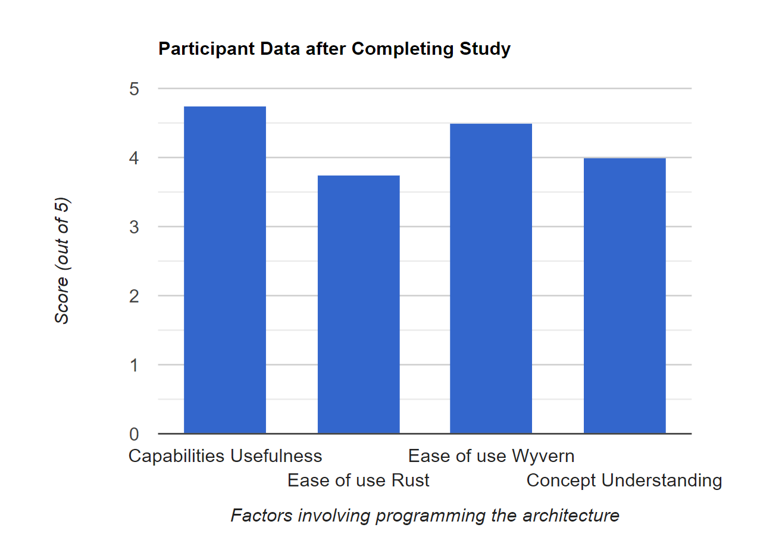
\includegraphics[width=2.1in]{figures/Quant_Results.png}
\caption{Quantitative Results for the Post-Study Survey (in order of questions asked in section \ref{sec:dataCollection}) }
\label{quantresults}
\end{figure}

\end{document}
